\part{Ubetinget Optimering}
\label{part:unconstrained_optimization}

\chapter{Teori og Problemformulering for Ubetinget Optimering}\label{chap:unconstrained_optimization}
Ubetinget optimalisering (eller fri optimalisering) refererer til problemer uten eksplisitte restriksjoner på variablene \(\symbf{x}\), eller løsningsmengden \(\Omega\).
Dette betyr at vi kan søke etter løsninger i hele \(\Omega = \R^n\) uten å måtte ta hensyn til begrensninger som kan hindre oss i å finne den beste løsningen.

\begin{example}{Eksempler på ubetinget optimering}{}
	Ubetinget optimering oppstår naturlig i mange praktiske problemer:

	\begin{itemize}
		\item \textbf{Tilpasning av modeller til data} (kurvetilpasning, regresjonsanalyse)
		\item \textbf{Maskinlæring} (trening av nevrale nettverk, logistisk regresjon)
		\item \textbf{Vitenskapelige beregninger} (simulering, minste kvadraters metode)
		\item \textbf{Bildebehandling} (filtrering, rekonstruksjon)
		\item \textbf{Økonomisk optimering} (porteføljeoptimering, kostnadsminimering)
	\end{itemize}

\end{example}

\section{Problemformulering og egenskaper}
Vi fokuserer nå på problemet med å minimere en \textit{objektfunksjon}
\( f : \R^n \to \R \) over hele rommet \(\R^n\):
\begin{mini*}|s|
	{\symbf{x} \in \R^n}{f(\symbf{x})}{}{\label{eq:global_minimization_problem}}
\end{mini*}

Den tillatte løsningsmengden omfatter hele \( \Omega = \R^n\).
Siden det ikke finnes restriksjoner å ta hensyn til, blir både problemet og løsningsmetodene enklere sammenlignet med betingede optimeringsproblemer.

Vi fokuserer hovedsakelig på minimering, men alle metoder kan anvendes på maksimeringsproblemer ved å minimere \(-f(\symbf{x})\), siden \(\max_{\symbf{x}} f(\symbf{x}) = -\min_{\symbf{x}} (-f(\symbf{x}))\).

I mange tilfeller kan også betingede optimeringsproblemer omformuleres som ubetingede problemer ved hjelp av straffefunksjoner eller barrierefunksjoner.

\section{Eksistens av løsninger}
\label{sec:existence_global_local_minimum}
I ubetinget optimering er det viktig å forstå eksistensen av minimum og hvordan de kan klassifiseres som lokale eller globale.

\subsection{Eksistens av Minimum}
\label{subsec:existence_of_minimum}

En grunnleggende spørsmål i ubetinget optimering er: Gitt en funksjon $f: \mathbb{R}^n \to \mathbb{R}$, finnes det et minimum av $f$ over $\mathbb{R}^n$? Svaret avhenger av egenskapene til $f$.

\begin{theorem}{Weierstrass' teorem}{weierstrass}
	Hvis $f: \mathbb{R}^n \to \mathbb{R}$ er kontinuerlig og det eksisterer en kompakt mengde $S \subset \mathbb{R}^n$ slik at
	\[
		\forall \symbf{x} \in \mathbb{R}^n \setminus S: f(\symbf{x}) > \inf_{\symbf{y} \in S} f(\symbf{y}),
	\]
	da har $f$ et globalt minimum på $\mathbb{R}^n$.
\end{theorem}

Dette teoremet garanterer eksistensen av et minimum når $f$ er kontinuerlig og på en eller annen måte "vokser" utenfor en begrenset mengde. En mer praktisk betingelse er koersivitet:

\begin{definition}{Koersiv funksjon}{coercive}
	En funksjon $f: \mathbb{R}^n \to \mathbb{R}$ er \emph{koersiv} hvis
	\[
		\lim_{\|\symbf{x}\| \to \infty} f(\symbf{x}) = \infty.
	\]
\end{definition}

\begin{proposition}{Eksistens av minimum for koersive funksjoner}{existence_coercive}
	La $f: \mathbb{R}^n \to \mathbb{R}$ være kontinuerlig og koersiv. Da har $f$ et globalt minimum på $\mathbb{R}^n$.
\end{proposition}

\begin{proof}
	Siden $f$ er koersiv, finnes det en $R > 0$ slik at $f(\symbf{x}) > f(\symbf{0})$ for alle $\|\symbf{x}\| > R$. La $S = \{\symbf{x} \in \mathbb{R}^n : \|\symbf{x}\| \leq R\}$. Da er $S$ kompakt, og vi vet at $\inf_{\symbf{y} \in \mathbb{R}^n} f(\symbf{y}) = \inf_{\symbf{y} \in S} f(\symbf{y})$. Fra Weierstrass' teorem, siden $f$ er kontinuerlig på den kompakte mengden $S$, oppnår $f$ et minimum på $S$. Dette minimumet er også et globalt minimum på $\mathbb{R}^n$.
\end{proof}

For konvekse funksjoner har vi følgende viktige resultat:

\begin{proposition}{Eksistens av minimum for konvekse funksjoner}{existence_convex}
	La $f: \mathbb{R}^n \to \mathbb{R}$ være en konveks funksjon som er nedenfra begrenset. Da har $f$ et globalt minimum hvis og bare hvis det finnes et stasjonært punkt $\symbf{x}^*$ slik at $\nabla f(\symbf{x}^*) = \symbf{0}$.
\end{proposition}

\begin{example}{Mangel på minimum}{no_minimum}
	Funksjonen $f(x) = e^{-x}$ oppnår ikke et minimum på $\mathbb{R}$ siden $\lim_{x \to \infty} f(x) = 0$, men $f(x) > 0$ for alle $x \in \mathbb{R}$.

	Tilsvarende har funksjonen $f(x, y) = x^2 + y^3$ ikke et globalt minimum, ettersom $\lim_{y \to -\infty} f(0, y) = -\infty$.
\end{example}

\begin{example}{Funksjoner med minimum}{with_minimum}
	\begin{itemize}
		\item Polynom med positiv ledende koeffisient (f.eks. $f(x) = x^2 + 3x - 2$) er koersiv og har dermed et globalt minimum.
		\item Normer og kvadratiske former $f(\symbf{x}) = \symbf{x}^T Q \symbf{x} + \symbf{b}^T \symbf{x} + c$ med $Q \succ 0$ (positiv definit) er konvekse og koersive, og har alltid et unikt globalt minimum.
	\end{itemize}
\end{example}

Oppsummert har vi følgende tilstrekkelige betingelser for eksistens av et minimum:
\begin{itemize}
	\item $f$ er kontinuerlig og koersiv
	\item $f$ er konveks, nedenfra begrenset, og har et stasjonært punkt
	\item $f$ er strengt konveks og nedenfra begrenset (garanterer et unikt globalt minimum)
\end{itemize}

\subsection{Lokale og Globale Minimum}
\label{sec:local_global_minimum}
Funksjoner kan ha flere ekstremalpunkter, og det er viktig å skille mellom lokale og globale minimum.
\begin{figure}[H]
	\centering
	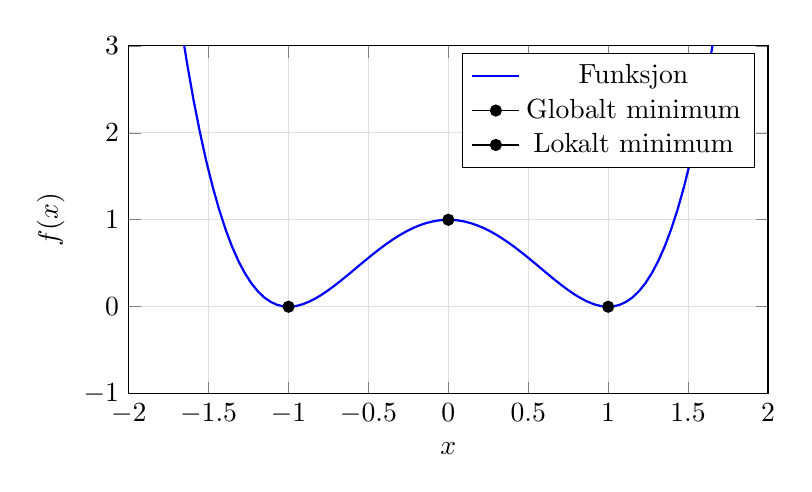
\begin{tikzpicture}
		\begin{axis}[
				xlabel={\(\symbf{x}\)},
				ylabel={\(f(\symbf{x})\)},
				xmin=-2, xmax=2,
				ymin=-1, ymax=3,
				width=0.8\textwidth,
				height=6cm,
				grid=both,
				minor grid style={gray!25},
				major grid style={gray!25}
			]
			\addplot[domain=-2:2, samples=100, thick, blue] {x^4 - 2*x^2 + 1};
			\addplot[mark=*] coordinates {(0, 1)};
			\addplot[mark=*] coordinates {(-1, 0)};
			\addplot[mark=*] coordinates {(1, 0)};
			\legend{Funksjon, Globalt minimum, Lokalt minimum}
		\end{axis}
	\end{tikzpicture}
	\caption{Eksempel på en funksjon med både lokale og globale ekstremalpunkter}
	\label{fig:local_vs_global}
\end{figure}
Funksjonen i figur \ref{fig:local_vs_global} har et globalt minimum i \((0, 1)\) og lokale minima i \((-1, 0)\) og \((1, 0)\).
\begin{definition}{Ekstremalpunkt}{extremum}
	Et punkt \(\symbf{x}^\ast \in \R^n\) er et \textit{ekstremalpunkt} for funksjonen \(f\) hvis det finnes en åpen omegn \(U\) rundt \(\symbf{x}^\ast\) slik at
	\[
		f(\symbf{x}^\ast) = f(\symbf{x}) \quad \text{for alle} \quad \symbf{x} \in U
	\]
\end{definition}
Ekstremalpunkter kan være enten maksimum eller minimum.

\begin{definition}{Lokalt maksimum}{local_maximum}
	Et punkt \(\symbf{x}^\ast \in \R^n\) er et \textit{lokalt maksimum} for funksjonen \(f\) hvis det finnes en åpen omegn \(U\) rundt \(\symbf{x}^\ast\) slik at
	\[
		f(\symbf{x}^\ast) \geq f(\symbf{x}) \quad \text{for alle} \quad \symbf{x} \in U
	\]
\end{definition}
\begin{definition}{Globalt maksimum}{global_maximum}
	Et punkt \(\symbf{x}^\ast \in \R^n\) er et \textit{globalt maksimum} for funksjonen \(f\) hvis
	\[
		f(\symbf{x}^\ast) \geq f(\symbf{x}) \quad \text{for alle} \quad \symbf{x} \in \R^n
	\]
\end{definition}

\begin{definition}{Globalt minimum}{global_minimum}
	Et punkt \(\symbf{x}^\ast \in \R^n\) er et \textit{globalt minimum} for funksjonen \(f\) hvis
	\[
		f(\symbf{x}^\ast) \leq f(\symbf{x}) \quad \text{for alle} \quad \symbf{x} \in \R^n
	\]
\end{definition}

\begin{definition}{Lokalt minimum}{local_minimum}
	Et punkt \(\symbf{x}^\ast \in \R^n\) er et \textit{lokalt minimum} for funksjonen \(f\) hvis det finnes en åpen omegn \(U\) rundt \(\symbf{x}^\ast\) slik at
	\[
		f(\symbf{x}^\ast) \leq f(\symbf{x}) \quad \text{for alle} \quad \symbf{x} \in U
	\]
\end{definition}

Vi sier at minimumet er \textit{strengt} hvis ulikhetene over holder strengt for alle \( \symbf{x} \neq \symbf{x}^\ast \).

Figur \ref{fig:local_vs_global} viser en funksjon med både lokale og globale ekstremalpunkter. I praksis er det generelt vanskelig å garantere at et funnet minimum er globalt, spesielt for ikke-konvekse funksjoner.

\subsection{Konveksitet i Ubetinget Optimering}
Konvekse funksjoner spiller en spesiell rolle i optimering fordi lokale minima også er globale minima.

\begin{definition}{Konveks funksjon}{convex_function}
	En funksjon \(f: \R^n \to \R\) er \textit{konveks} hvis for alle \(\symbf{x}, \symbf{y} \in \R^n\) og alle \(\lambda \in [0,1]\) gjelder
	\[
		f(\lambda \symbf{x} + (1-\lambda)\symbf{y}) \leq \lambda f(\symbf{x}) + (1-\lambda)f(\symbf{y})
	\]
	Funksjonen er \textit{strengt konveks} hvis ulikheten over er streng for alle \(\symbf{x} \neq \symbf{y}\) og \(\lambda \in (0,1)\).
\end{definition}

For differensierbare funksjoner har vi følgende karakterisering:

\begin{proposition}{Karakterisering av differensierbare konvekse funksjoner}{differentiable_convex}
	La \(f: \R^n \to \R\) være en differensierbar funksjon. Da er \(f\) konveks hvis og bare hvis for alle \(\symbf{x}, \symbf{y} \in \R^n\) gjelder
	\[
		f(\symbf{y}) \geq f(\symbf{x}) + \nabla f(\symbf{x})^T (\symbf{y} - \symbf{x})
	\]
\end{proposition}

For to ganger differensierbare funksjoner har vi en enda enklere karakterisering:

\begin{proposition}{Karakterisering med Hesse-matrisen}{hessian_convex}
	La \(f: \R^n \to \R\) være to ganger kontinuerlig differensierbar. Da er \(f\) konveks hvis og bare hvis Hesse-matrisen \(\nabla^2 f(\symbf{x})\) er positiv semidefinit for alle \(\symbf{x} \in \R^n\).

	Funksjonen er strengt konveks hvis og bare hvis Hesse-matrisen er positiv definit for alle \(\symbf{x} \in \R^n\).
\end{proposition}

\section{Stasjonære Punkter}
\label{sec:stationary_points}

\subsection{Definisjon og egenskaper}
\label{subsec:stationary_def_prop}

Stasjonære punkter spiller en sentral rolle i optimeringsteori og representerer potensielle kandidater for optimale løsninger.

\begin{definition}{Stasjonært punkt}{stationary_point}
	Et punkt \(\symbf{x}^\ast \in \R^n\) kalles et \textit{stasjonært punkt} for \(f\) hvis \(f\) er differensierbar ved \(\symbf{x}^\ast\) og
	\[
		\nabla f(\symbf{x}^\ast) = \symbf{0}
	\]
\end{definition}

Stasjonære punkter har følgende viktige egenskaper:
\begin{itemize}
	\item De er nødvendige (men ikke tilstrekkelige) betingelser for lokale ekstremalpunkter
	\item De representerer punkter der den deriverte forsvinner i alle retninger
	\item De inkluderer alle lokale minima, maksima og sadelpunkter
\end{itemize}

Et stasjonært punkt kan klassifiseres som:
\begin{itemize}
	\item Et \textit{lokalt minimum}: Funksjonsverdien er mindre enn eller lik verdien i nærliggende punkter
	\item Et \textit{lokalt maksimum}: Funksjonsverdien er større enn eller lik verdien i nærliggende punkter
	\item Et \textit{sadelpunkt}: Punktet er verken et lokalt minimum eller maksimum
\end{itemize}

Fra et geometrisk perspektiv representerer stasjonære punkter steder der tangentplanet til funksjonen er horisontalt.

\subsection{Gradient og Hessian}
\label{subsec:gradient_hessian}

For å analysere stasjonære punkter bruker vi både gradienten og Hesse-matrisen.

\begin{itemize}
	\item \textbf{Gradienten} \(\nabla f(\symbf{x})\) angir retningen med bratteste stigning ved punktet \(\symbf{x}\)
	\item \textbf{Hesse-matrisen} \(\nabla^2 f(\symbf{x})\) inneholder andreordens partiellderiverte og beskriver kurvaturinformasjonen av \(f\) ved punktet \(\symbf{x}\)
\end{itemize}

Ved et stasjonært punkt \(\symbf{x}^\ast\) hvor \(\nabla f(\symbf{x}^\ast) = \symbf{0}\), kan vi bruke Hesse-matrisen til å bestemme punktets natur:

\begin{table}[H]
	\centering
	\begin{tabular}{|c|c|}
		\hline
		\textbf{Egenskaper ved \(\nabla^2 f(\symbf{x}^\ast)\)} & \textbf{Klassifisering av \(\symbf{x}^\ast\)} \\
		\hline
		Positiv definit                                        & Strengt lokalt minimum                        \\
		\hline
		Positiv semidefinit                                    & Lokalt minimum (ikke nødvendigvis strengt)    \\
		\hline
		Negativ definit                                        & Strengt lokalt maksimum                       \\
		\hline
		Negativ semidefinit                                    & Lokalt maksimum (ikke nødvendigvis strengt)   \\
		\hline
		Indefinit (verken positiv eller negativ semidefinit)   & Sadelpunkt                                    \\
		\hline
	\end{tabular}
	\caption{Klassifisering av stasjonære punkter basert på Hesse-matrisen}
	\label{tab:stationary_classification}
\end{table}

\subsection{Stasjonære punkter i flere dimensjoner}
\label{subsec:stationary_multi_dim}

I én dimensjon er karakterisering av stasjonære punkter relativt enkel:
\begin{itemize}
	\item hvis \(f''(x^\ast) > 0\), har vi et lokalt minimum
	\item hvis \(f''(x^\ast) < 0\), har vi et lokalt maksimum
	\item hvis \(f''(x^\ast) = 0\), er ytterligere analyse nødvendig
\end{itemize}

I flere dimensjoner blir situasjonen mer kompleks. Sadelpunkter oppstår ofte, og karakteriseringen avhenger av egenverdiene til Hesse-matrisen.

\begin{example}{Stasjonære punkter i to dimensjoner}{stationary_2d}
	Betrakt funksjonen \(f(x,y) = x^2 + y^2 - 4xy\). De stasjonære punktene finnes ved å løse:
	\begin{align*}
		\nabla f(x,y) = \begin{pmatrix} 2x - 4y \\ 2y - 4x \end{pmatrix} = \begin{pmatrix} 0 \\ 0 \end{pmatrix}
	\end{align*}
	Dette gir \(x = y = 0\). Hesse-matrisen er:
	\begin{align*}
		\nabla^2 f(x,y) = \begin{pmatrix} 2 & -4 \\ -4 & 2 \end{pmatrix}
	\end{align*}
	Egenverdiene er \(\lambda_1 = 6\) og \(\lambda_2 = -2\), noe som indikerer at \((0,0)\) er et sadelpunkt.
\end{example}

En funksjon i \(n\) dimensjoner kan ha langt flere stasjonære punkter enn i én dimensjon, og de kan være vanskeligere å finne analytisk. I høyere dimensjoner blir sannsynligheten for sadelpunkter større enn sannsynligheten for lokale minima, noe som har betydelige implikasjoner for optimeringsalgoritmer.

For å oppsummere:
\begin{itemize}
	\item I én dimensjon: stasjonære punkter er enten lokale minima, lokale maksima eller vendepunkter
	\item I to dimensjoner: stasjonære punkter kan være lokale minima, lokale maksima eller sadelpunkter
	\item I \(n\) dimensjoner: et stasjonært punkt kan ha enhver kombinasjon av positiv, negativ og null kurvatur i forskjellige retninger
\end{itemize}

\section{Optimalitetsbetingelser}

\subsection{Førsteordens Nødvendige Betingelse}

\begin{theorem}{Førsteordens nødvendige betingelse}{first_order_necessary}
	Anta at \(f: \R^n \to \R\) er kontinuerlig differensierbar og at \(\symbf{x}^\ast\) er et lokalt minimum for \(f\). Da er \(\symbf{x}^\ast\) et stasjonært punkt, dvs.
	\[
		\nabla f(\symbf{x}^\ast) = \symbf{0}
	\]
\end{theorem}

\subsection{Andreordens Betingelser (Nødvendige og Tilstrekkelige)}

\begin{theorem}{Andreordens nødvendige betingelse}{second_order_necessary}
	Anta at \(f: \R^n \to \R\) er to ganger kontinuerlig differensierbar og at \(\symbf{x}^\ast\) er et lokalt minimum for \(f\). Da er Hesse-matrisen \(\nabla^2 f(\symbf{x}^\ast)\) positiv semidefinit.
\end{theorem}

\begin{theorem}{Andreordens tilstrekkelig betingelse}{second_order_sufficient}
	Anta at \(f: \R^n \to \R\) er to ganger kontinuerlig differensierbar, \(\nabla f(\symbf{x}^\ast) = \symbf{0}\) og Hesse-matrisen \(\nabla^2 f(\symbf{x}^\ast)\) er positiv definit. Da er \(\symbf{x}^\ast\) et strengt lokalt minimum for \(f\).
\end{theorem}

\section{Konvergens}
\label{sec:convergence_theory}

Konvergens er et fundamentalt konsept i optimering som beskriver hvordan en sekvens av iterasjoner \(\{\symbf{x}_k\}\) oppfører seg etter hvert som algoritmen skrider frem. Når vi analyserer konvergens, er vi interessert i hvorvidt -- og hvordan -- algoritmen nærmer seg en løsning.

\subsection{Global og lokal konvergens}

En viktig distinksjon i konvergensteori er skillet mellom global og lokal konvergens.

\begin{definition}{Global konvergens}{global_convergence}
	En algoritme er \emph{globalt konvergent} hvis sekvensen \(\{\symbf{x}_k\}\) konvergerer til en stasjonær punkt \(\symbf{x}^\ast\) (der \(\nabla f(\symbf{x}^\ast) = \symbf{0}\)) uansett valg av startpunkt \(\symbf{x}_0\).
\end{definition}

\begin{definition}{Lokal konvergens}{local_convergence}
	En algoritme er \emph{lokalt konvergent} hvis sekvensen \(\{\symbf{x}_k\}\) konvergerer til et stasjonært punkt \(\symbf{x}^\ast\) når startpunktet \(\symbf{x}_0\) er tilstrekkelig nær \(\symbf{x}^\ast\).
\end{definition}

Mange kraftige algoritmer, som Newtons metode, har bare lokal konvergensgaranti. Dette er en av grunnene til at vi trenger globaliseringsstrategier som linjesøk og tillitsregion-metoder.

\subsection{Konvergenskriterier}

For å avgjøre om en algoritme har konvergert i praksis, bruker vi ulike stoppekriterier:

\begin{enumerate}
	\item \textbf{Gradientnorm}: \(\|\nabla f(\symbf{x}_k)\| < \epsilon_g\) for en liten toleranse \(\epsilon_g > 0\).
	\item \textbf{Iterasjonsendring}: \(\|\symbf{x}_{k+1} - \symbf{x}_k\| < \epsilon_x\) for en liten toleranse \(\epsilon_x > 0\).
	\item \textbf{Funksjonsendring}: \(|f(\symbf{x}_{k+1}) - f(\symbf{x}_k)| < \epsilon_f\) for en liten toleranse \(\epsilon_f > 0\).
	\item \textbf{Maksimalt antall iterasjoner}: \(k > k_{\max}\).
\end{enumerate}

En kombinasjon av disse kriteriene brukes ofte for å sikre robust konvergens. Det første kriteriet er særlig viktig siden det direkte tester om vi har nådd et stasjonært punkt.

\subsection{Konvergensbetingelser}

For iterative algoritmer på formen \(\symbf{x}_{k+1} = \symbf{x}_k + \alpha_k \symbf{d}_k\), har vi følgende viktige betingelser for konvergens:

\begin{theorem}{Konvergensbetingelser for nedstigningsalgoritmer}{descent_method_convergence}
	La \(f: \mathbb{R}^n \to \mathbb{R}\) være kontinuerlig deriverbar og nedenfra begrenset. En iterativ algoritme på formen \(\symbf{x}_{k+1} = \symbf{x}_k + \alpha_k \symbf{d}_k\) konvergerer til et stasjonært punkt hvis følgende betingelser er oppfylt:
	\begin{enumerate}
		\item Retningen \(\symbf{d}_k\) er en nedstigningsretning, dvs. \(\nabla f(\symbf{x}_k)^T\symbf{d}_k < 0\) så lenge \(\nabla f(\symbf{x}_k) \neq \symbf{0}\).
		\item Steglengden \(\alpha_k\) velges slik at den tilfredsstiller tilstrekkelig reduksjonsbetingelse, f.eks. Armijo-betingelsen.
		\item Retningene er gradientrelaterte, dvs. det finnes konstanter \(c_1, c_2 > 0\) slik at
		      \[
			      c_1 \|\nabla f(\symbf{x}_k)\| \leq \|\symbf{d}_k\| \leq c_2 \|\nabla f(\symbf{x}_k)\|
		      \]
		      for alle \(k\).
	\end{enumerate}
\end{theorem}

\begin{proof}
	En skisse av beviset følger Zoutendijk's teorem, som viser at
	\[
		\sum_{k=0}^{\infty} \cos^2 \theta_k \|\nabla f(\symbf{x}_k)\|^2 < \infty,
	\]
	hvor \(\theta_k\) er vinkelen mellom \(\symbf{d}_k\) og \(-\nabla f(\symbf{x}_k)\). Gradientrelasjonen sikrer at \(\cos \theta_k\) er nedenfra begrenset vekk fra null, noe som impliserer at \(\|\nabla f(\symbf{x}_k)\| \to 0\).
\end{proof}

\subsection{Eksempler på konvergente og ikke-konvergente sekvenser}

\begin{example}{Konvergent sekvens med gradientmetode}{convergent_gradient}
	Betrakt funksjonen \(f(x) = x^2\) og gradientmetoden \(x_{k+1} = x_k - \alpha_k \nabla f(x_k)\) med fast steglengde \(\alpha_k = \alpha = 0.5\). Med startpunkt \(x_0 = 1\) får vi:
	\[
		\begin{array}{l|l|l}
			k & x_k    & \nabla f(x_k) \\
			\hline
			0 & 1.0000 & 2.0000        \\
			1 & 0.0000 & 0.0000        \\
		\end{array}
	\]
	Her konvergerer sekvensen i én iterasjon siden \(\alpha = 0.5 = 1/(2 \cdot 1)\) er den optimale steglengden for denne funksjonen.
\end{example}

\begin{example}{Ikke-konvergent sekvens}{non_convergent}
	Betrakt samme funksjon \(f(x) = x^2\), men med steglengde \(\alpha_k = \alpha = 1.0\). Med startpunkt \(x_0 = 1\) får vi:
	\[
		\begin{array}{l|l|l}
			k      & x_k     & \nabla f(x_k) \\
			\hline
			0      & 1.0000  & 2.0000        \\
			1      & -1.0000 & -2.0000       \\
			2      & 1.0000  & 2.0000        \\
			\vdots & \vdots  & \vdots        \\
		\end{array}
	\]
	Her oscillerer sekvensen mellom 1 og -1 og konvergerer ikke, fordi steglengden er for stor.
\end{example}

\begin{example}{Zigzag-konvergens}{zigzag_convergence}
	Betrakt funksjonen \(f(x, y) = 100(y - x^2)^2 + (1 - x)^2\) (Rosenbrock-funksjonen) og gradientmetoden med fast steglengde. Denne funksjonen er kjent for å føre til "zigzag"-konvergens der algoritmen tar mange små skritt langs dalbunnen, noe som resulterer i langsom konvergens til minimumet ved \((1, 1)\).
\end{example}

\section{Konvergenshastighet}
\label{sec:convergence_rates}

Konvergenshastighet beskriver hvor raskt en sekvens \(\{\symbf{x}_k\}\) nærmer seg løsningen \(\symbf{x}^\ast\). Dette er avgjørende for å forstå effektiviteten til forskjellige optimeringsalgoritmer.

\begin{definition}{Konvergensrater}{convergence_rates}
	Anta at sekvensen \(\{\symbf{x}_k\}\) konvergerer mot \(\symbf{x}^\ast\). Vi sier at konvergensen er:
	\begin{itemize}
		\item \textbf{Lineær} hvis det finnes en konstant \(r \in (0,1)\) slik at
		      \[
			      \lim_{k \to \infty} \frac{\|\symbf{x}_{k+1} - \symbf{x}^\ast\|}{\|\symbf{x}_k - \symbf{x}^\ast\|} = r
		      \]

		\item \textbf{Superlineær} hvis
		      \[
			      \lim_{k \to \infty} \frac{\|\symbf{x}_{k+1} - \symbf{x}^\ast\|}{\|\symbf{x}_k - \symbf{x}^\ast\|} = 0
		      \]

		\item \textbf{Kvadratisk} hvis det finnes en konstant \(M > 0\) slik at
		      \[
			      \lim_{k \to \infty} \frac{\|\symbf{x}_{k+1} - \symbf{x}^\ast\|}{\|\symbf{x}_k - \symbf{x}^\ast\|^2} = M
		      \]

		\item \textbf{Sublineær} hvis for en \(p \in (0,1)\), det finnes en konstant \(C > 0\) slik at
		      \[
			      \|\symbf{x}_{k} - \symbf{x}^\ast\| \leq \frac{C}{k^p}
		      \]
	\end{itemize}
\end{definition}

\subsection{Lineær konvergens}

Lineær konvergens betyr at feilen reduseres med en konstant faktor i hver iterasjon. For en lineært konvergent sekvens kan vi skrive:
\[
	\|\symbf{x}_{k+1} - \symbf{x}^\ast\| \leq r \|\symbf{x}_k - \symbf{x}^\ast\|, \quad 0 < r < 1
\]
Dette gir en feilreduksjon på formen \(\|\symbf{x}_k - \symbf{x}^\ast\| \leq r^k \|\symbf{x}_0 - \symbf{x}^\ast\|\).

Mange førsteordens metoder, som gradientmetoden med fast steglengde, har lineær konvergenshastighet. Konvergensfaktoren \(r\) avhenger ofte av problemets kondisjonering:

\begin{proposition}{Konvergensfaktor for gradientmetoden}{gradient_convergence_factor}
	For en kvadratisk funksjon \(f(\symbf{x}) = \frac{1}{2}\symbf{x}^T\symbf{Q}\symbf{x} - \symbf{b}^T\symbf{x}\) med positiv definitt matrise \(\symbf{Q}\), konvergerer gradientmetoden med optimal steglengde lineært med faktor
	\[
		r = \frac{\kappa - 1}{\kappa + 1}
	\]
	hvor \(\kappa = \lambda_{\max}/\lambda_{\min}\) er kondisjonstallet til \(\symbf{Q}\).
\end{proposition}

\subsection{Superlineær konvergens}

Superlineær konvergens er raskere enn lineær, men langsommere enn kvadratisk. Den karakteriseres ved:
\[
	\lim_{k \to \infty} \frac{\|\symbf{x}_{k+1} - \symbf{x}^\ast\|}{\|\symbf{x}_k - \symbf{x}^\ast\|} = 0
\]

Dette betyr at konvergenshastigheten akselererer etter hvert som vi nærmer oss løsningen. Kvasi-Newton-metoder som BFGS oppnår vanligvis superlineær konvergens fordi de bygger opp en stadig mer nøyaktig tilnærming til den inverse Hessian-matrisen.

\subsection{Kvadratisk konvergens}

Kvadratisk konvergens er den raskeste av de vanlige konvergensratene og karakteriseres ved:
\[
	\|\symbf{x}_{k+1} - \symbf{x}^\ast\| \leq M \|\symbf{x}_k - \symbf{x}^\ast\|^2
\]
for en konstant \(M > 0\).

Dette gir en dramatisk økning i presisjon, der antallet korrekte sifre omtrent dobles i hver iterasjon. Newtons metode oppviser kvadratisk konvergens nær løsningen når følgende betingelser er oppfylt:
\begin{itemize}
	\item Funksjonen \(f\) er to ganger kontinuerlig deriverbar i en omegn av \(\symbf{x}^\ast\).
	\item Hesse-matrisen \(\nabla^2 f(\symbf{x}^\ast)\) er positiv definitt.
	\item Startpunktet \(\symbf{x}_0\) er tilstrekkelig nær \(\symbf{x}^\ast\).
\end{itemize}

\begin{theorem}{Kvadratisk konvergens av Newtons metode}{newton_quadratic_convergence}
	La \(f: \mathbb{R}^n \to \mathbb{R}\) være to ganger kontinuerlig deriverbar i en åpen mengde som inneholder et lokalt minimum \(\symbf{x}^\ast\). Anta at Hesse-matrisen \(\nabla^2 f(\symbf{x}^\ast)\) er positiv definitt og Lipschitz-kontinuerlig i en omegn av \(\symbf{x}^\ast\). Da finnes en \(\delta > 0\) slik at for alle \(\symbf{x}_0\) med \(\|\symbf{x}_0 - \symbf{x}^\ast\| < \delta\), konvergerer Newtons metode
	\[
		\symbf{x}_{k+1} = \symbf{x}_k - [\nabla^2 f(\symbf{x}_k)]^{-1}\nabla f(\symbf{x}_k)
	\]
	kvadratisk mot \(\symbf{x}^\ast\).
\end{theorem}

\subsection{Sammenligning av konvergensrater}

\begin{figure}[H]
	\centering
	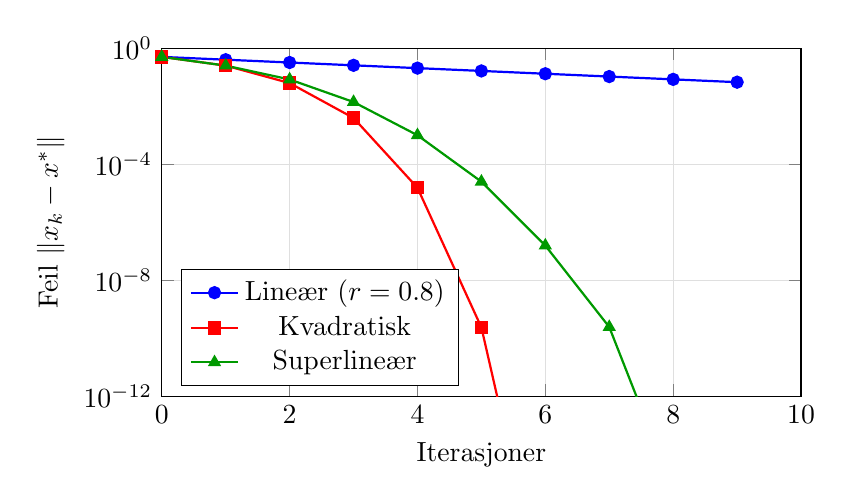
\begin{tikzpicture}
		\begin{semilogyaxis}[
				xlabel={Iterasjoner},
				ylabel={Feil \( \|\symbf{x}_k - \symbf{x}^\ast\| \)},
				xmin=0, xmax=10,
				ymin=1e-12, ymax=1,
				width=0.8\textwidth,
				height=6cm,
				legend pos=south west,
				grid=both,
				minor grid style={gray!25},
				major grid style={gray!25}
			]
			\addplot[blue, thick, mark=*] coordinates {
					(0, 0.5)
					(1, 0.4)
					(2, 0.32)
					(3, 0.256)
					(4, 0.2048)
					(5, 0.16384)
					(6, 0.131072)
					(7, 0.1048576)
					(8, 0.08388608)
					(9, 0.067108864)
				};
			\addlegendentry{Lineær (\( r=0.8 \))}

			\addplot[red, thick, mark=square*] coordinates {
					(0, 0.5)
					(1, 0.25)
					(2, 0.0625)
					(3, 0.00390625)
					(4, 1.52588e-5)
					(5, 2.32831e-10)
					(6, 5.42101e-20)
					(7, 2.93873e-39)
					(8, 8.63617e-78)
					(9, 7.45832e-155)
				};
			\addlegendentry{Kvadratisk}

			\addplot[green!60!black, thick, mark=triangle*] coordinates {
					(0, 0.5)
					(1, 0.25)
					(2, 0.0833333)
					(3, 0.0138889)
					(4, 0.000992063)
					(5, 2.48016e-5)
					(6, 1.55009e-7)
					(7, 2.40637e-10)
					(8, 5.79065e-16)
					(9, 3.35458e-27)
				};
			\addlegendentry{Superlineær}

		\end{semilogyaxis}
	\end{tikzpicture}
	\caption{Sammenligning av konvergensrater: lineær, superlineær og kvadratisk konvergens}
	\label{fig:convergence_rates}
\end{figure}

Figur \ref{fig:convergence_rates} illustrerer de dramatiske forskjellene mellom ulike konvergensrater. Merk at:

\begin{itemize}
	\item Med lineær konvergens reduseres feilen med samme faktor i hver iterasjon.
	\item Med superlineær konvergens akselererer konvergenshastigheten over tid.
	\item Med kvadratisk konvergens dobles antallet riktige sifre omtrent i hver iterasjon.
\end{itemize}

I praksis er antallet iterasjoner som kreves for å nå en gitt toleranse \(\epsilon\) avhengig av konvergensraten:

\begin{itemize}
	\item Lineær: \(k \approx \log_{1/r}(\|\symbf{x}_0 - \symbf{x}^\ast\|/\epsilon)\)
	\item Kvadratisk: \(k \approx \log_2(\log_2(\|\symbf{x}_0 - \symbf{x}^\ast\|/\epsilon))\)
\end{itemize}

\subsection{Faktorer som påvirker konvergenshastigheten}

Flere faktorer kan påvirke konvergenshastigheten til optimeringsalgoritmer:

\begin{enumerate}
	\item \textbf{Problemets kondisjonering}: Høyt kondisjonstall \(\kappa\) reduserer konvergenshastigheten, særlig for førsteordens metoder.

	\item \textbf{Funksjonens glatthet}: Ikke-glatte funksjoner fører til langsommere konvergens fordi differensieringsegenskaper er begrenset.

	\item \textbf{Startpunktets kvalitet}: Et startpunkt nær løsningen forbedrer konvergensen, spesielt for lokalt konvergente metoder som Newton.

	\item \textbf{Problemets dimensjonalitet}: Høydimensjonale problemer kan være vanskeligere å konvergere for på grunn av større søkerom.

	\item \textbf{Parametrisering og skalering}: Dårlig skalerte variabler kan føre til langsommere konvergens.
\end{enumerate}

\begin{example}{Prekondisjonering}{preconditioning}
	Prekondisjonering kan dramatisk forbedre konvergenshastigheten for dårlig kondisjonerte problemer. For eksempel, ved å løse
	\[
		\symbf{P}^{-1}\symbf{A}\symbf{x} = \symbf{P}^{-1}\symbf{b}
	\]
	med en egnet prekondisjonerer \(\symbf{P}\) som approksimerer \(\symbf{A}\), kan vi redusere kondisjonstallet og dermed akselerere konvergensen.
\end{example}

\begin{table}[H]
	\centering
	\begin{tabular}{|l|c|c|c|}
		\hline
		\textbf{Metode}            & \textbf{Konvergensrate} & \textbf{Minne} & \textbf{Beregningskostnad/iter.} \\
		\hline
		Gradient (fast steglengde) & Lineær                  & \(O(n)\)       & \(O(n)\)                         \\
		Gradient (eksakt linjesøk) & Lineær                  & \(O(n)\)       & \(O(n) + \) linjesøk             \\
		Newton                     & Kvadratisk              & \(O(n^2)\)     & \(O(n^3)\)                       \\
		BFGS                       & Superlineær             & \(O(n^2)\)     & \(O(n^2)\)                       \\
		L-BFGS                     & Superlineær             & \(O(mN)\)      & \(O(mN)\)                        \\
		Konjugert Gradient         & Superlineær/Lineær      & \(O(n)\)       & \(O(n) + \) linjesøk             \\
		\hline
	\end{tabular}
	\caption{Sammenligning av optimeringsmetoder med hensyn til konvergensrate og ressursbehov}
	\label{tab:method_comparison}
\end{table}

Tabell \ref{tab:method_comparison} sammenligner ulike optimeringsmetoder med hensyn til deres konvergensrater og ressursbehov. Valget av algoritme involverer en avveiing mellom konvergenshastighet og beregningsmessig kostnad per iterasjon.

\section{Taylor-ekspansjoner}
\label{sec:taylor_expansion}

Taylor-ekspansjoner er viktig i optimeringsteorien fordi de gir lokale approksimasjoner av en funksjon rundt et punkt. De utgjør det matematiske grunnlaget for mange optimeringsalgoritmer, spesielt gradientbaserte metoder.

\subsection{Taylor-ekspansjon for funksjoner av én variabel}

For en funksjon $f: \mathbb{R} \to \mathbb{R}$ som er $n$ ganger kontinuerlig deriverbar i et punkt $a$, er Taylor-polynomet av grad $n$ rundt $a$ gitt ved:

\begin{equation}
	P_n(x) = \sum_{k=0}^{n} \frac{f^{(k)}(a)}{k!}(x-a)^k = f(a) + f'(a)(x-a) + \frac{f''(a)}{2}(x-a)^2 + \cdots + \frac{f^{(n)}(a)}{n!}(x-a)^n
\end{equation}

Hvis $f$ er $(n+1)$ ganger kontinuerlig deriverbar, kan feilen i approksimasjonen uttrykkes ved:

\begin{equation}
	f(x) = P_n(x) + R_n(x)
\end{equation}

hvor restleddet $R_n(x)$ er gitt ved:

\begin{equation}
	R_n(x) = \frac{f^{(n+1)}(\xi)}{(n+1)!}(x-a)^{n+1}
\end{equation}

for en $\xi$ mellom $a$ og $x$.

\subsection{Taylor-ekspansjon for flervariable funksjoner}

For en funksjon $f: \mathbb{R}^n \to \mathbb{R}$ som er tilstrekkelig glatt, kan vi utvide konseptet til flere variabler. La $\symbf{x}, \symbf{a} \in \mathbb{R}^n$. Første- og andreordens Taylor-ekspansjoner er da gitt ved:

\begin{align}
	f(\symbf{x}) & \approx f(\symbf{a}) + \nabla f(\symbf{a})^T(\symbf{x}-\symbf{a})                                                                                \\
	f(\symbf{x}) & \approx f(\symbf{a}) + \nabla f(\symbf{a})^T(\symbf{x}-\symbf{a}) + \frac{1}{2}(\symbf{x}-\symbf{a})^T\nabla^2 f(\symbf{a})(\symbf{x}-\symbf{a})
\end{align}

hvor $\nabla f(\symbf{a})$ er gradienten av $f$ ved $\symbf{a}$ og $\nabla^2 f(\symbf{a})$ er Hesse-matrisen.

\subsection{Taylor-ekspansjoner i optimering}

Taylor-ekspansjoner er sentrale i optimering av flere grunner:

\begin{enumerate}
	\item \textbf{Første-ordens metoder}: Gradientnedstigningsmetoder bruker en lineær (første-ordens) Taylor-approksimasjon for å bestemme søkeretningen:
	      \begin{equation}
		      f(\symbf{x}_k + \symbf{p}) \approx f(\symbf{x}_k) + \nabla f(\symbf{x}_k)^T\symbf{p}
	      \end{equation}
	      Retningen $\symbf{p} = -\nabla f(\symbf{x}_k)$ minimerer denne approksimasjonen.

	\item \textbf{Andre-ordens metoder}: Newtons metode bruker andre-ordens Taylor-approksimasjon:
	      \begin{equation}
		      f(\symbf{x}_k + \symbf{p}) \approx f(\symbf{x}_k) + \nabla f(\symbf{x}_k)^T\symbf{p} + \frac{1}{2}\symbf{p}^T\nabla^2 f(\symbf{x}_k)\symbf{p}
	      \end{equation}
	      Retningen $\symbf{p} = -[\nabla^2 f(\symbf{x}_k)]^{-1}\nabla f(\symbf{x}_k)$ minimerer denne approksimasjonen.

	\item \textbf{Kvasi-Newton-metoder}: Disse metodene bruker også andre-ordens Taylor-approksimasjoner, men med en approksimert Hesse-matrise som oppdateres iterativt.

	\item \textbf{Trust region-metoder}: Disse metodene minimerer en Taylor-approksimasjon innenfor et bestemt område (trust region) hvor approksimeringen antas å være gyldig.
\end{enumerate}

\subsection{Nøyaktighet og konvergenshastighet}

Nøyaktigheten av Taylor-ekspansjonen påvirker direkte konvergenshastigheten til optimeringsalgoritmer:

\begin{itemize}
	\item \textbf{Første-ordens metoder} (f.eks. gradientnedstigningen) oppnår lineær konvergens under passende betingelser.
	\item \textbf{Andre-ordens metoder} (f.eks. Newtons metode) kan oppnå kvadratisk konvergens i nærheten av et minimum.
\end{itemize}

\begin{example}{Taylor-approksimasjon for optimeringsproblemer}{taylor_approx_opt}
	Betrakt funksjonen $f(x) = e^x - x$. Vi ønsker å finne minimumspunktet ved å bruke Newtons metode, som er basert på andre-ordens Taylor-approksimasjon.

	Vi starter med et punkt $x_0 = 0$. Ved dette punktet er:
	\begin{align*}
		f(0)   & = 1           \\
		f'(0)  & = e^0 - 1 = 0 \\
		f''(0) & = e^0 = 1
	\end{align*}

	Andre-ordens Taylor-approksimasjonen rundt $x_0 = 0$ er:
	\[
		f(x) \approx 1 + 0 \cdot (x-0) + \frac{1}{2} \cdot 1 \cdot (x-0)^2 = 1 + \frac{x^2}{2}
	\]

	Denne approksimasjonen har et minimum ved $x = 0$, som tilfeldigvis er et stasjonært punkt for den opprinnelige funksjonen. Siden $f'(0) = 0$ og $f''(0) > 0$, er dette faktisk et lokalt minimum.
\end{example}

\begin{example}{Newton-steg basert på Taylor-ekspansjon}{newton_step_taylor}
	Betrakt funksjonen $f(x) = x^4 - 4x^2 + 2$. Vi ønsker å finne et minimum ved å bruke Newtons metode, som utgår fra andre-ordens Taylor-ekspansjoner.

	Vi starter med et punkt $x_0 = 1$. Ved dette punktet er:
	\begin{align*}
		f'(1)  & = 4x^3 - 8x|_{x=1} = 4 - 8 = -4 \\
		f''(1) & = 12x^2 - 8|_{x=1} = 12 - 8 = 4
	\end{align*}

	Andre-ordens Taylor-approksimasjonen rundt $x_0 = 1$ er:
	\[
		f(x) \approx f(1) + f'(1)(x-1) + \frac{1}{2}f''(1)(x-1)^2 = -1 - 4(x-1) + 2(x-1)^2
	\]

	For å finne det neste Newton-steget, minimerer vi denne approksimasjonen ved å sette den deriverte lik null:
	\[
		\frac{d}{dx}[-1 - 4(x-1) + 2(x-1)^2] = -4 + 4(x-1) = 0
	\]

	Dette gir $x-1 = 1$ eller $x = 2$. Dermed er neste punkt i Newtons metode $x_1 = 2$.

	De faktiske stasjonære punktene for $f(x) = x^4 - 4x^2 + 2$ er $x = \pm \sqrt{2}$. Med flere Newton-steg vil algoritmen konvergere mot det nærmeste stasjonære punktet, som i dette tilfellet er $x = \sqrt{2} \approx 1.414$.
\end{example}

Taylor-ekspansjoner gir altså en måte å tilnærme en funksjon lokalt, noe som muliggjør utvikling av effektive optimeringsalgoritmer. Valget av hvilken orden Taylor-ekspansjon som brukes, påvirker både beregningsmessig kostnad og konvergenshastighet for algoritmene.

\chapter{Algoritmer for ubetinget optimering}
\label{chap:iterative_methods}

De fleste optimeringsproblemer løses ikke analytisk, men ved hjelp av iterative metoder som gradvis nærmer seg en optimal løsning.
Dette kapittelet beskriver grunnleggende iterative metoder for ubetinget optimering, med særlig fokus på hvordan ulike søkeretninger påvirker ytelsen til disse metodene.

\section{Algoritmestruktur}
\label{sec:iterative_structure}

Iterative metoder for ubetinget optimering følger typisk en felles struktur: start med et initialgjett, beregn en søkeretning, ta et steg i denne retningen, og gjenta prosessen til konvergens er oppnådd.

\begin{algorithm}[H]
	\SetAlgoLined
	\KwIn{Startpunkt \(\symbf{x}_0\), toleranse \(\epsilon > 0\)}
	\KwOut{Omtrentlig løsning \(\symbf{x}^\ast\)}
	\For{\(k = 0, 1, 2, \ldots\)}{
		\If{\(\|\nabla f(\symbf{x}_k)\| < \epsilon\)}{
			\Return{\(\symbf{x}_k\)}
		}
		Beregn søkeretning \(\symbf{d}_k\)\;
		Bestem steglengde \(\alpha_k\)\;
		Oppdater \(\symbf{x}_{k+1} = \symbf{x}_k + \alpha_k\symbf{d}_k\)\;
	}
	\caption{Grunnleggende iterativ optimeringsalgoritme}
	\label{alg:general_iterative}
\end{algorithm}

Avgjørende for algoritmens effektivitet er valg av søkeretning \(\symbf{d}_k\) og steglengde \(\alpha_k\). Sammen bestemmer disse hvor neste iterasjon plasseres og dermed hvorvidt algoritmen konvergerer raskt, langsomt eller ikke i det hele tatt.
\subsection{Nedstigningsretninger}
\label{sec:descent_directions}

For at en iterativ metode skal være effektiv, må søkeretningen føre til en reduksjon i objektfunksjonen. Dette konseptet formaliseres gjennom begrepet nedstigningsretning.

\begin{definition}{Nedstigningsretning}{descent_direction}
	En vektor \(\symbf{d}\) er en \emph{nedstigningsretning} for funksjonen \(f\) ved punktet \(\symbf{x}\) hvis det eksisterer et \(\bar{\alpha} > 0\) slik at
	\[
		f(\symbf{x} + \alpha\symbf{d}) < f(\symbf{x}) \quad \text{for alle } \alpha \in (0,\bar{\alpha}]
	\]
\end{definition}

For differensierbare funksjoner har vi en enkel karakterisering av nedstigningsretninger:

\begin{proposition}{Karakterisering av nedstigningsretninger}{descent_direction_char}
	For en kontinuerlig deriverbar funksjon \(f\) er \(\symbf{d}\) en nedstigningsretning ved \(\symbf{x}\) hvis og bare hvis
	\[
		\nabla f(\symbf{x})^T\symbf{d} < 0
	\]
\end{proposition}

\begin{proof}{}{}
	Ved å bruke Taylor-ekspansjonen av første orden får vi:
	\[
		f(\symbf{x} + \alpha\symbf{d}) = f(\symbf{x}) + \alpha \nabla f(\symbf{x})^T\symbf{d} + o(\alpha)
	\]

	For tilstrekkelig små \(\alpha > 0\) vil fortegnet til \(f(\symbf{x} + \alpha\symbf{d}) - f(\symbf{x})\) bestemmes av leddet \(\alpha \nabla f(\symbf{x})^T\symbf{d}\). Dette leddet er negativt hvis og bare hvis \(\nabla f(\symbf{x})^T\symbf{d} < 0\).
\end{proof}

\section{Søkeretninger}
\label{sec:key_search_directions}

Det finnes mange måter å velge nedstigningsretninger på. Vi skal nå se på de tre mest sentrale:
\begin{itemize}
	\item Gradientretningen (steepest descent)
	\item Newtonretningen
	\item Kvasi-Newton retninger
\end{itemize}

\subsection{Gradientretningen (steepest descent)}
\label{subsec:steepest_descent}

Den enkleste og mest intuitive nedstigningsretningen er den negative gradienten:
\[
	\symbf{d}_k = -\nabla f(\symbf{x}_k)
\]

Denne retningen har følgende egenskaper:
\begin{itemize}
	\item Den gir den bratteste nedstigning lokalt (derav navnet "steepest descent")
	\item Den er enkel og rimelig å beregne, med kun behov for førsteordens derivasjoner
	\item Den konvergerer lineært, og kan være svært langsom for dårlig kondisjonerte problemer
	\item Den kan vise "zigzag"-oppførsel, hvor påfølgende retninger oscillerer i stedet for å bevege seg direkte mot løsningen
\end{itemize}


\subsection{Newtonretningen}
\label{subsec:newton_direction}

Newtonretningen bruker andreordens informasjon for å ta hensyn til funksjoners krumning:
\[
	\symbf{d}_k = -[\nabla^2 f(\symbf{x}_k)]^{-1}\nabla f(\symbf{x}_k)
\]

Denne retningen har følgende egenskaper:
\begin{itemize}
	\item Den gir kvadratisk konvergens nær løsningen når Hesse-matrisen er positiv definit
	\item Den er beregningsmessig krevende, spesielt i høyere dimensjoner
	\item Den krever eksplisitt beregning og inversjon av Hesse-matrisen
	\item Den er sårbar for problemer når Hesse-matrisen ikke er positiv definit
\end{itemize}

\subsection{Kvasi-Newton retninger}
\label{subsec:quasi_newton_directions}

Kvasi-Newton metoder forsøker å få "det beste fra begge verdener" ved å approksimere Hesse-matrisen uten å beregne den eksplisitt:
\[
	\symbf{d}_k = -\symbf{B}_k^{-1}\nabla f(\symbf{x}_k)
\]

hvor \(\symbf{B}_k\) er en approksimasjon av Hesse-matrisen som bygges opp gjennom iterative oppdateringer.

Disse metodene har følgende egenskaper:
\begin{itemize}
	\item De gir superlineær konvergens under passende betingelser
	\item De unngår eksplisitt beregning av Hesse-matrisen
	\item De balanserer beregningsmessig kostnad mot konvergenshastighet
	\item Populære varianter inkluderer BFGS, DFP og L-BFGS
\end{itemize}

\subsection{Hvordan velge søkeretning?}
\label{sec:search_direction_choice}
Valget av søkeretning avhenger av flere faktorer, inkludert problemets dimensjon, regneressurser og ønsket nøyaktighet.

\begin{table}[H]
	\centering
	\begin{tabular}{lcccl}
		\toprule
		\textbf{Metode} & \textbf{Konvergensrate} & \textbf{Kostnad/iter} & \textbf{Minnekrav} & \textbf{Egnet for}                           \\
		\midrule
		Gradient        & Lineær                  & O(n)                  & O(n)               & Store problemer, begrensede ressurser        \\
		Newton          & Kvadratisk              & O(n³)                 & O(n²)              & Små til mellomstore problemer, høy presisjon \\
		Kvasi-Newton    & Superlineær             & O(n²)                 & O(n²)              & Mellomstore problemer, balansert ytelse      \\
		\bottomrule
	\end{tabular}
	\caption{Sammenligning av ulike søkeretninger}
	\label{tab:search_direction_comparison}
\end{table}

\subsection{Praktiske strategier}
\label{subsec:practical_strategies}

I praksis kombineres ofte ulike søkeretninger:

\begin{itemize}
	\item \textbf{Hybride metoder}: Start med gradientmetoden for robusthet, bytt til Newton eller kvasi-Newton når man nærmer seg løsningen
	\item \textbf{Prekondisjonering}: Forbedre konvergensen til gradientmetoden ved å skalere variablene eller transformere problemet
	\item \textbf{Linje- og tillitsregionsøk}: Benytt sofistikerte teknikker for å velge steglengde som sikrer global konvergens
	\item \textbf{Regularisering}: Modifiser Hesse-matrisen (f.eks. ved å legge til en identitetsmatrise) for å sikre positiv definithet
\end{itemize}

Optimering i praksis innebærer å velge riktig søkeretningsstrategi basert på problemets struktur og tilgjengelige ressurser. Mens gradientmetoden er enkel og robust, kan Newton og kvasi-Newton-metoder gi betydelig raskere konvergens for passende problemer.

\chapter{Steglengdemetoder}
\label{chap:step_length_methods}
Steglengdemetoder er en viktig del av optimeringsalgoritmer, spesielt i gradientbaserte metoder som Newtons metode og Quasi-Newton-metoder.

De har som mål å bestemme den optimale steglengden \(\alpha\) for å minimere objektfunksjonen \(f\) langs en gitt retning \(p\).

\section{Linjesøk-metoder}
\label{sec:line_search_methods}

Linjesøk-metoder er en metode for å finne den optimale steglengden \(\alpha_k\) i iterative optimeringsalgoritmer.
Disse metodene er avgjørende for å sikre at algoritmen konvergerer mot en løsning på en effektiv måte.
Hovedideen er å først velge en nedstigningsretning \(\symbf{d}_k\), og deretter finne en steglengde \(\alpha_k > 0\) som gir tilstrekkelig reduksjon i objektfunksjonen.

\begin{definition}{Linjesøk}{line_search}
	Gitt en nåværende iterasjon \(\symbf{x}_k\) og en søkeretning \(\symbf{d}_k\), finner linjesøk en steglengde \(\alpha_k > 0\) slik at
	\[
		\symbf{x}_{k+1} = \symbf{x}_k + \alpha_k \symbf{d}_k
	\]
	gir tilstrekkelig reduksjon i \(f\) langs retningen \(\symbf{d}_k\).
\end{definition}

\begin{figure}[H]
	\centering
	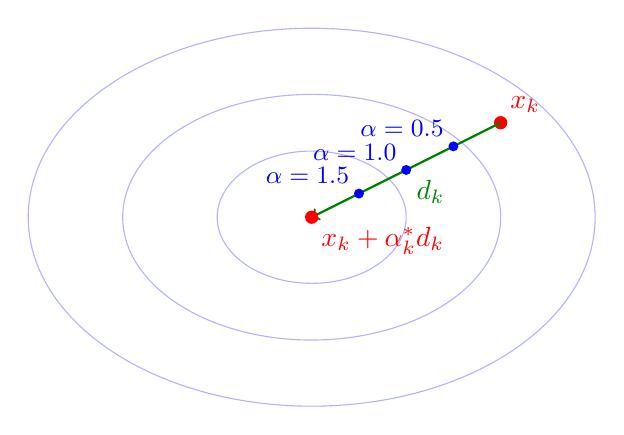
\begin{tikzpicture}[scale=1.2]
		% Contour lines - centered at origin
		\draw[blue!30] (0,0) ellipse (3 and 2);
		\draw[blue!30] (0,0) ellipse (2 and 1.3);
		\draw[blue!30] (0,0) ellipse (1 and 0.7);

		% Current point
		\fill[red] (2,1) circle (2pt) node[above right] {$\symbf{x}_k$};

		% Search direction - now points to origin (minimum)
		\draw[->, thick, green!50!black] (2,1) -- (0,0) node[midway, below right] {$\symbf{d}_k$};

		% Step points along the path to minimum
		\fill[blue] (1.5,0.75) circle (1.5pt) node[above left,font=\small] {$\alpha=0.5$};
		\fill[blue] (1,0.5) circle (1.5pt) node[above left,font=\small] {$\alpha=1.0$};
		\fill[blue] (0.5,0.25) circle (1.5pt) node[above left,font=\small] {$\alpha=1.5$};

		% Minimum point
		\fill[red] (0,0) circle (2pt) node[below right] {$\symbf{x}_k + \alpha_k^* \symbf{d}_k$};
	\end{tikzpicture}
	\caption{Linjesøk langs en nedstigningsretning $\symbf{d}_k$ fra et punkt $\symbf{x}_k$. Forskjellige steglengder $\alpha$ gir forskjellige kandidatpunkter, og den optimale steglengden $\alpha_k^*$ fører til minimumet ved origo.}
	\label{fig:line_search_illustration}
\end{figure}

For å oppnå god konvergens, må steglengden \(\alpha_k\) oppfylle visse betingelser.
Disse betingelsene varierer i hvor strenge krav de stiller til reduksjonen i funksjonsverdien, gradientens/Hesse-matrisens oppførsel og forholdet mellom disse.
De mest kjente er Armijo-betingelsen, Wolfe-betingelsene, Strong Wolfe-betingelsene, Goldstein-betingelsene og kurvbetingelsen.

Det er viktig å merke seg at linjesøk kan være en kostbar operasjon, spesielt i høyere dimensjoner.

Det finnes to typer av linjesøk:
\begin{itemize}
	\item \textbf{Eksakt linjesøk}: Finn \( \alpha_k \) som minimerer \( f(\symbf{x}_k + \alpha \symbf{d}_k) \). Dette er ofte beregningsmessig dyrt.
	\item \textbf{Ikke-eksakt linjesøk}: Finn \( \alpha_k \) som gir tilstrekkelig reduksjon ved å oppfylle visse betingelser, som Wolfe-betingelsene.
\end{itemize}

\subsection{Eksakte linjesøk}
\label{subsec:exact_line_search}

Eksakt linjesøk innebærer å finne den aller beste steglengden \(\alpha_k\) som minimerer funksjonen \(f\) langs den valgte nedstigningsretningen \(\symbf{d}_k\).

\begin{definition}{Eksakt linjesøk}{exact_line_search}
	Gitt en nåværende iterasjon \(\symbf{x}_k\) og en nedstigningsretning \(\symbf{d}_k\), er den eksakte linjesøk-løsningen \(\alpha_k^\star\) gitt ved:
	\[
		\alpha_k^\star = \arg\min_{\alpha > 0} f(\symbf{x}_k + \alpha \symbf{d}_k)
	\]
	Dette innebærer å løse et én-dimensjonalt optimeringsproblem.
\end{definition}
Eksakt linjesøk er ofte beregningsmessig kostbart, særlig for høydimensjonale problemer. Det er likevel viktig å forstå prinsippene bak og når det kan være fordelaktig å bruke.

\subsubsection{Eksempler på eksakt linjesøk}
\label{subsubsec:exact_line_search_examples}

\begin{example}{Eksakt linjesøk for kvadratiske funksjoner}{exact_line_search_quadratic}
	For kvadratiske funksjoner kan vi beregne den optimale steglengden analytisk. Gitt en funksjon på formen
	$f(\symbf{x}) = \frac{1}{2}\symbf{x}^T\symbf{Q}\symbf{x} - \symbf{b}^T\symbf{x} + c$ med positiv definitt $\symbf{Q}$,
	er den optimale steglengden:

	\begin{equation*}
		\alpha_k = \frac{\symbf{d}_k^T(\symbf{b} - \symbf{Q}\symbf{x}_k)}{\symbf{d}_k^T\symbf{Q}\symbf{d}_k} = \frac{-\symbf{d}_k^T\nabla f(\symbf{x}_k)}{\symbf{d}_k^T\symbf{Q}\symbf{d}_k}
	\end{equation*}

	Denne formelen avhenger kun av gradienten $\nabla f(\symbf{x}_k) = \symbf{Q}\symbf{x}_k - \symbf{b}$ og
	søkeretningen $\symbf{d}_k$.

	% 3D-plot
	\begin{center}
		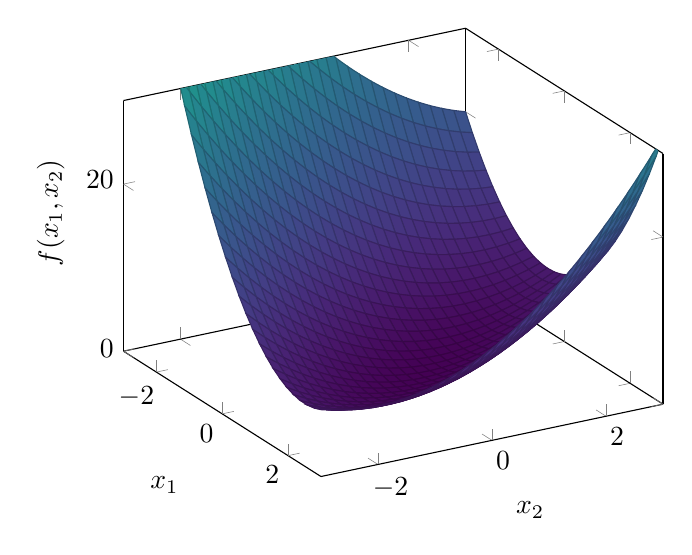
\begin{tikzpicture}
			\begin{axis}[
					view={60}{30},
					xlabel={$x_1$},
					ylabel={$x_2$},
					zlabel={$f(x_1,x_2)$},
					xmin=-3, xmax=3,
					ymin=-3, ymax=3,
					zmin=0, zmax=30,
					samples=30,
					domain=-3:3,
				]
				\addplot3[surf, mesh/rows=30, colormap/viridis] {2*x^2 + y^2 + 2*x*y - 4*x - 2*y + 5};
			\end{axis}

		\end{tikzpicture}
	\end{center}
\end{example}


\begin{example}{Konkret beregning av eksakt linjesøk}{exact_line_search_numerical}
	Betrakt den kvadratiske funksjonen $f(x,y) = 2x^2 + y^2 + 2xy - 4x - 2y + 5$ med startpunktet
	$\symbf{x}_0 = (0,0)^T$ og søkeretningen $\symbf{d}_0 = (-1,-1)^T$. Vi kan finne den optimale steglengden analytisk.

	Vi identifiserer først matrise- og vektorparametrene:
	\[
		\symbf{Q} = \begin{bmatrix} 4 & 2 \\ 2 & 2 \end{bmatrix}, \quad
		\symbf{b} = \begin{bmatrix} 4 \\ 2 \end{bmatrix}, \quad
		c = 5
	\]

	Ved startpunktet $\symbf{x}_0 = (0,0)^T$ er gradienten $\nabla f(\symbf{x}_0) = \symbf{Q}\symbf{x}_0 - \symbf{b} = -\symbf{b} = (-4,-2)^T$.

	Den optimale steglengden blir:
	\begin{align*}
		\alpha_0 & = \frac{-\symbf{d}_0^T\nabla f(\symbf{x}_0)}{\symbf{d}_0^T\symbf{Q}\symbf{d}_0}               \\
		         & = \frac{-(-1,-1)\cdot(-4,-2)^T}{(-1,-1)\begin{bmatrix} 4 & 2 \\ 2 & 2 \end{bmatrix}(-1,-1)^T} \\
		         & = \frac{6}{10} = 0.6
	\end{align*}

	Det neste punktet i optimeringsprosessen blir dermed
	$\symbf{x}_1 = \symbf{x}_0 + \alpha_0 \symbf{d}_0 = (0,0) + 0.6 \cdot (-1,-1) = (-0.6, -0.6)$.
\end{example}

I praksis er eksakt linjesøk ofte for beregningsmessig kostbart for generelle funksjoner, og vi bruker derfor ikke-eksakte metoder som garanterer tilstrekkelig reduksjon uten å finne det eksakte minimumet.

\subsection{Ikke-eksakte linjesøk}
\label{subsec:inexact_line_search}
Ikke-eksakte linjesøk-metoder finner en steglengde \(\alpha_k\) som tilfredsstiller visse betingelser, uten å nødvendigvis minimere funksjonen eksakt.
Disse betingelsene sikrer at steglengden er tilstrekkelig for å oppnå en betydelig reduksjon i objektfunksjonen, samtidig som den unngår de beregningsmessige kostnadene ved eksakte metoder.

Det finnes flere varianter av ikke-eksakte linjesøk-metoder.

\subsubsection{Armijo-betingelsen}
\label{subsubsec:armijo_condition}

Den mest grunnleggende betingelsen er Armijo-betingelsen, som sikrer tilstrekkelig reduksjon i funksjonsverdien:

\begin{definition}{Armijo-betingelsen}{armijo_condition}
	En steglengde \(\alpha\) tilfredsstiller Armijo-betingelsen hvis:
	\begin{equation}\label{eq:armijo_condition}
		f(\symbf{x}_k + \alpha \symbf{d}_k)
		\leq
		f(\symbf{x}_k)
		+
		c_1\alpha\nabla f(\symbf{x}_k)^T \symbf{d}_k,
	\end{equation}
	hvor \(c_1 \in (0,1)\) er en liten konstant, typisk \(c_1 \approx 10^{-4}\). Dette sikrer at funksjonen reduseres minst like mye som en fraksjon av den lineære prediksjonen.
\end{definition}

\begin{figure}[H]
	\centering
	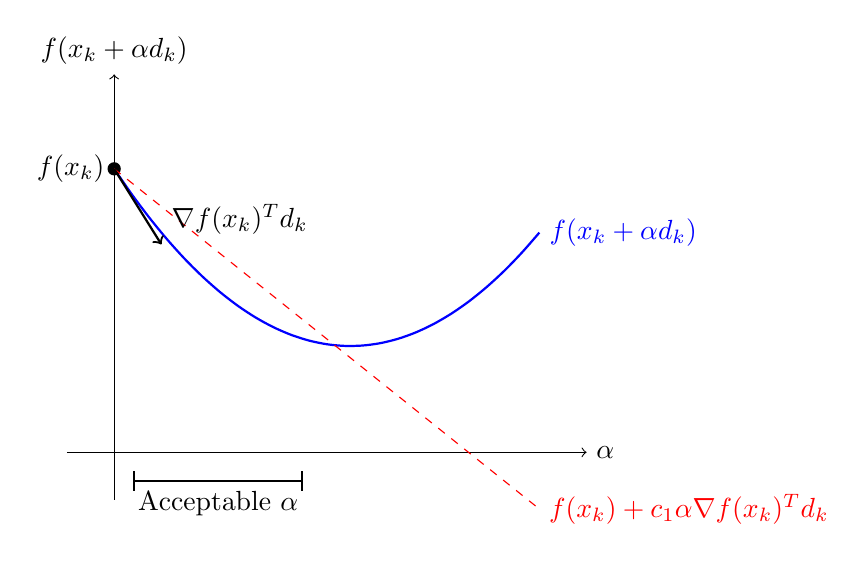
\begin{tikzpicture}[scale=1.2]
		% Axes
		\draw[->] (-0.5,0) -- (5,0) node[right]{$\alpha$};
		\draw[->] (0,-0.5) -- (0,4) node[above]{$f(\symbf{x}_k + \alpha\symbf{d}_k)$};

		% Function curve
		\draw[thick, blue] plot[domain=0:4.5, smooth] (\x,{3-1.5*\x+0.3*\x*\x}) node[right]{$f(\symbf{x}_k + \alpha\symbf{d}_k)$};

		% Initial point
		\fill (0,3) circle (2pt) node[left] {$f(\symbf{x}_k)$};

		% Armijo line
		\draw[red, dashed, domain=0:4.5] plot (\x,{3-0.8*\x}) node[right]{$f(\symbf{x}_k) + c_1\alpha\nabla f(\symbf{x}_k)^T\symbf{d}_k$};

		% Gradient at initial point
		\draw[->, thick] (0,3) -- (0.5,2.2) node[above right] {$\nabla f(\symbf{x}_k)^T\symbf{d}_k$};

		% Acceptable region
		\draw[|-|, thick] (0.2,-0.3) -- (2,-0.3) node[midway, below] {Acceptable $\alpha$};

	\end{tikzpicture}
	\caption{Armijo-betingelsen: Den blå kurven viser objektfunksjonen langs søkeretningen, mens den røde stiplede linjen viser den øvre grensen gitt av Armijo-betingelsen. Alle steglengder $\alpha$ hvor den blå kurven ligger under den røde linjen er akseptable.}
	\label{fig:armijo_condition}
\end{figure}
Armijo-betingelsen sikrer en tilstrekkelig reduksjon, men garanterer ikke at steglengden er lang nok. For korte steglengder kan føre til svært små fremskritt og langsom konvergens, noe som kalles "Maratos-effekten". Dette problemet løses ved å legge til tilleggsbetingelser.

\subsubsection{Krumningsbetingelse}
\label{subsubsec:curvature_condition}
Krumningsbetingelsen (\emph{curvature condition}) er en tilleggsbetingelse som sikrer at steglengden ikke er for kort.
Den krever at gradienten langs søkeretningen har blitt mindre negativ, noe som indikerer at vi har beveget oss forbi en region med bratt nedstigning.

\begin{definition}{Curvature condition}{curvature_condition}
	En steglengde \(\alpha\) tilfredsstiller kurvbetingelsen hvis:
	\begin{equation}\label{eq:curvature_condition}
		c_2 \nabla f(\symbf{x}_k)^T \symbf{d}_k \leq \nabla f(\symbf{x}_k + \alpha \symbf{d}_k)^T \symbf{d}_k
	\end{equation}
	hvor \(c_2 \in (c_1, 1)\), typisk \(c_2 \approx 0.9\).
\end{definition}

Kurvbetingelsen sikrer at gradienten langs søkeretningen har blitt mindre negativ, noe som indikerer at vi har beveget oss forbi en region med bratt nedstigning.

\subsubsection{Wolfe-betingelsene}
\label{subsubsec:wolfe_conditions}

Kombinasjonen av Armijo-betingelsen \ref{def:armijo_condition} og kurvbetingelsen \ref{def:curvature_condition} gir Wolfe-betingelsene.

\begin{definition}{Wolfe-betingelsene}{wolfe_conditions}
	En steglengde \(\alpha\) tilfredsstiller Wolfe-betingelsene hvis:
	\begin{align}
		f(\symbf{x}_k + \alpha\symbf{d}_k)    & \leq f(\symbf{x}_k) + c_1\alpha\nabla f(\symbf{x}_k)^T\symbf{d}_k \tag{(Armijo)}    \\
		c_2\nabla f(\symbf{x}_k)^T\symbf{d}_k & \leq \nabla f(\symbf{x}_k + \alpha\symbf{d}_k)^T\symbf{d}_k  \tag{(Kurvbetingelse)}
	\end{align}
	hvor \(0 < c_1 < c_2 < 1\).
\end{definition}

\begin{figure}[H]
	\centering
	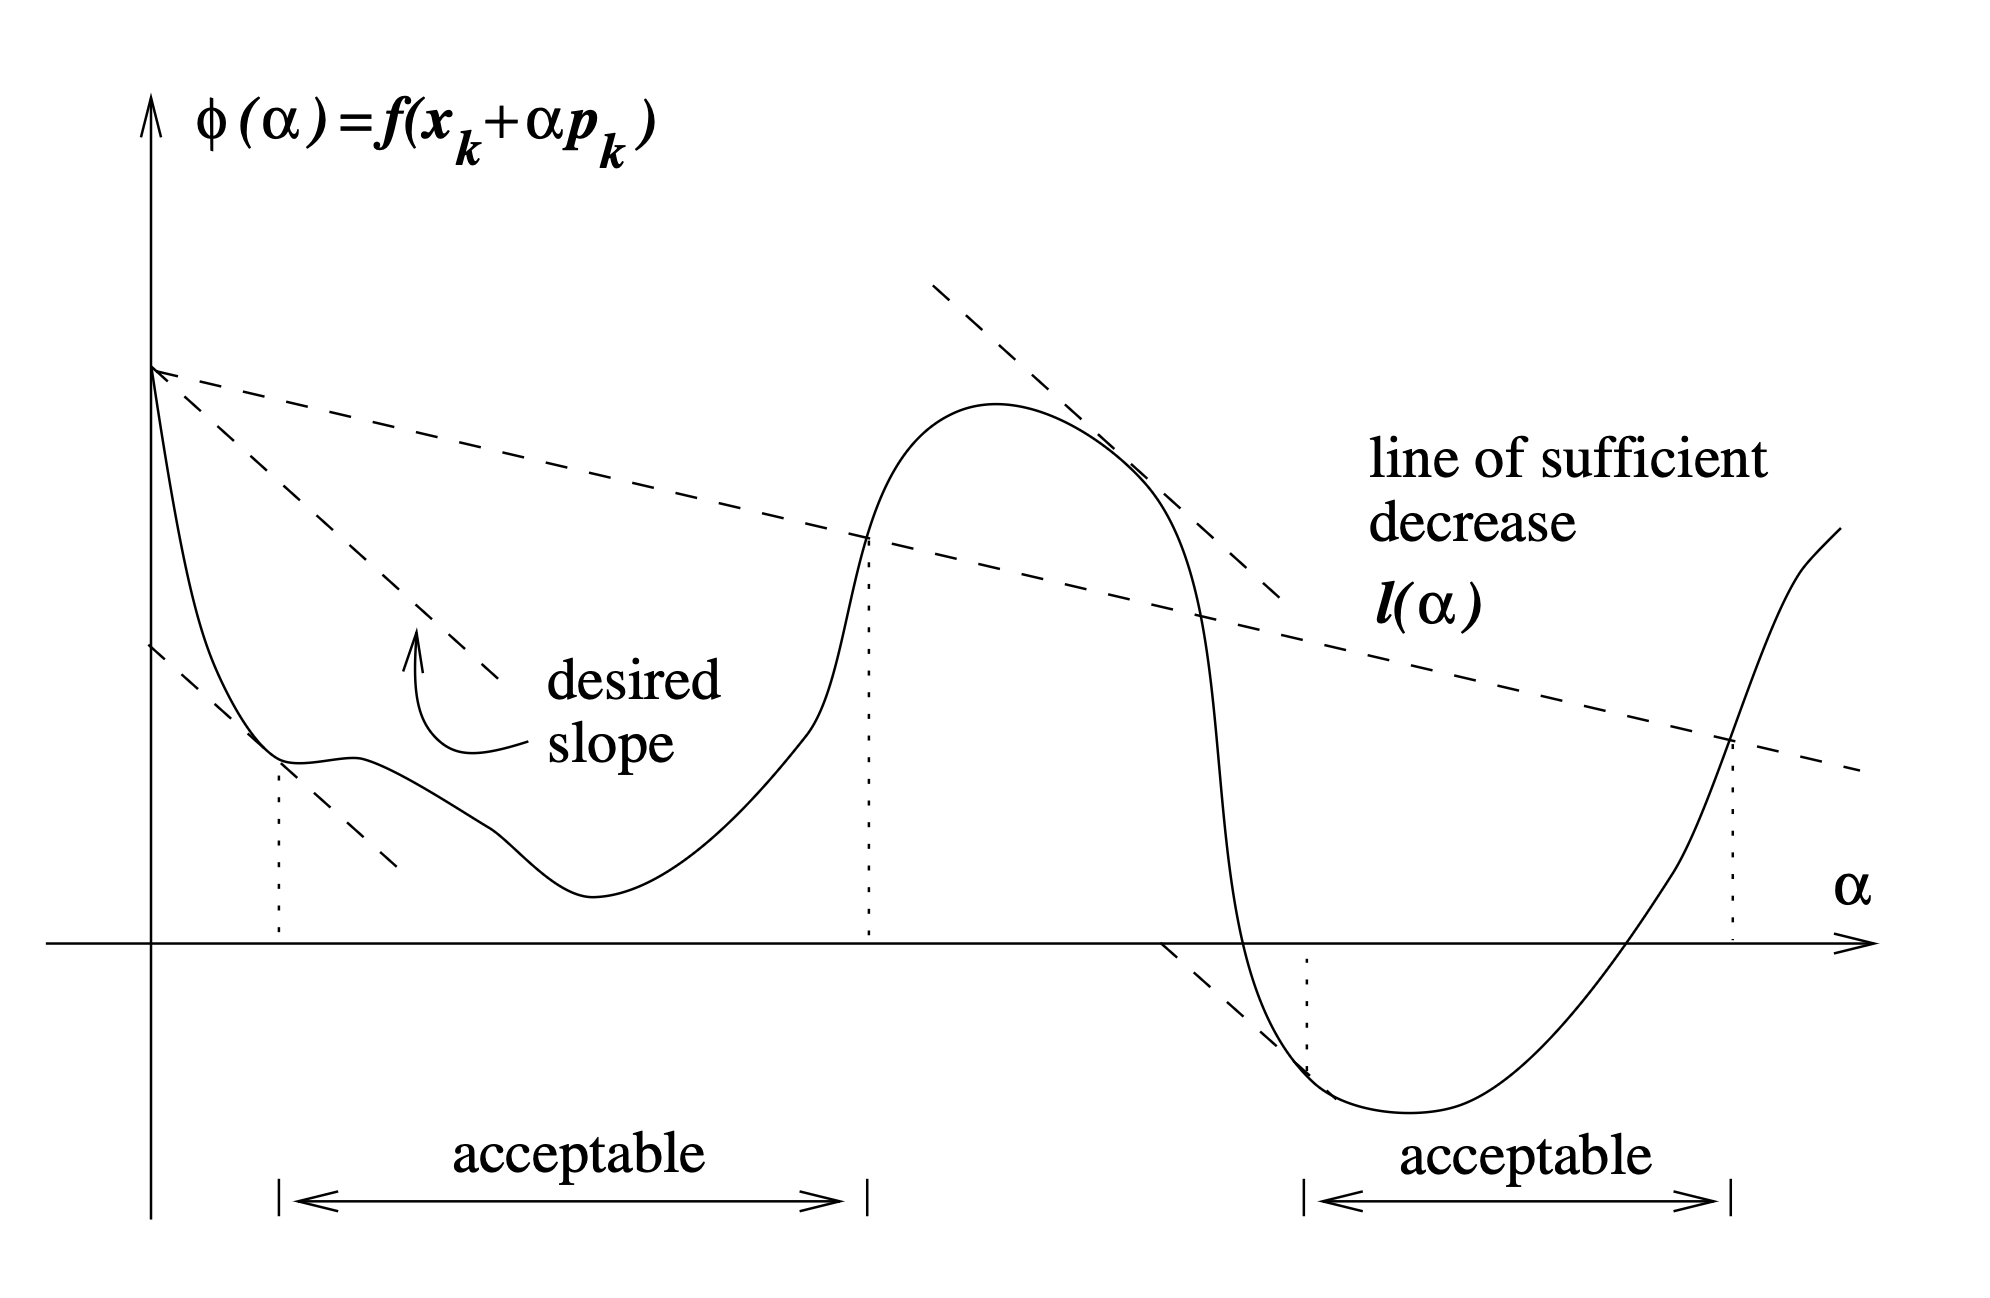
\includegraphics[width=0.8\textwidth]{figures/wolfe_conditions.png}
	\caption{Wolfe-betingelsene}
	\label{fig:wolfe_conditions}
\end{figure}

\subsubsection{Strong Wolfe-betingelsene}
\label{subsubsec:strong_wolfe_conditions}
For visse algoritmer, som konjugerte gradientmetoder, er det nyttig med en strengere betingelse som også begrenser gradientens absolutte størrelse:

\begin{definition}{Strong Wolfe-betingelsene}{strong_wolfe_conditions}
	En steglengde \(\alpha\) tilfredsstiller de sterke Wolfe-betingelsene hvis:
	\begin{align}
		f(\symbf{x}_k + \alpha_k\symbf{p}_k)                       & \leq f(\symbf{x}_k) + c_1\alpha_k\nabla f(\symbf{x}_k)^T\symbf{p}_k \\
		|\nabla f(\symbf{x}_k + \alpha_k\symbf{p}_k)^T\symbf{p}_k| & \leq c_2|\nabla f(\symbf{x}_k)^T\symbf{p}_k|
	\end{align}
	hvor \(0 < c_1 < c_2 < 1\), typisk er $c_1 \approx 10^{-4}$ og $c_2 \approx 0.9$.
\end{definition}

Den andre betingelsen i de sterke Wolfe-betingelsene sikrer at gradienten langs søkeretningen er liten i absoluttverdi, noe som hindrer at algoritmen tar for store steg når gradienten skifter fortegn.

\subsubsection{Goldstein-betingelsene}
\label{subsubsec:goldstein_conditions}

En alternativ tilnærming til Wolfe-betingelsene er Goldstein-betingelsene, som danner et intervall rundt den lineære approksimasjonen:
\[
	f(\symbf{x}_k + \alpha\symbf{d}_k) \approx f(\symbf{x}_k) + \alpha\nabla f(\symbf{x}_k)^T\symbf{d}_k
\]

\begin{definition}{Goldstein-betingelsene}{goldstein_conditions}
	En steglengde \(\alpha\) tilfredsstiller Goldstein-betingelsene hvis:
	\begin{equation}\label{eq:goldstein_conditions}
		f(\symbf{x}_k) + (1-c)\alpha\nabla f(\symbf{x}_k)^T\symbf{d}_k  \leq f(\symbf{x}_k + \alpha\symbf{d}_k) \leq f(\symbf{x}_k) + c\alpha\nabla f(\symbf{x}_k)^T\symbf{d}_k
	\end{equation}
	hvor \(c \in (0, \frac{1}{2})\), typisk \(c = 10^{-4}\).
\end{definition}
\begin{figure}[H]
	\centering
	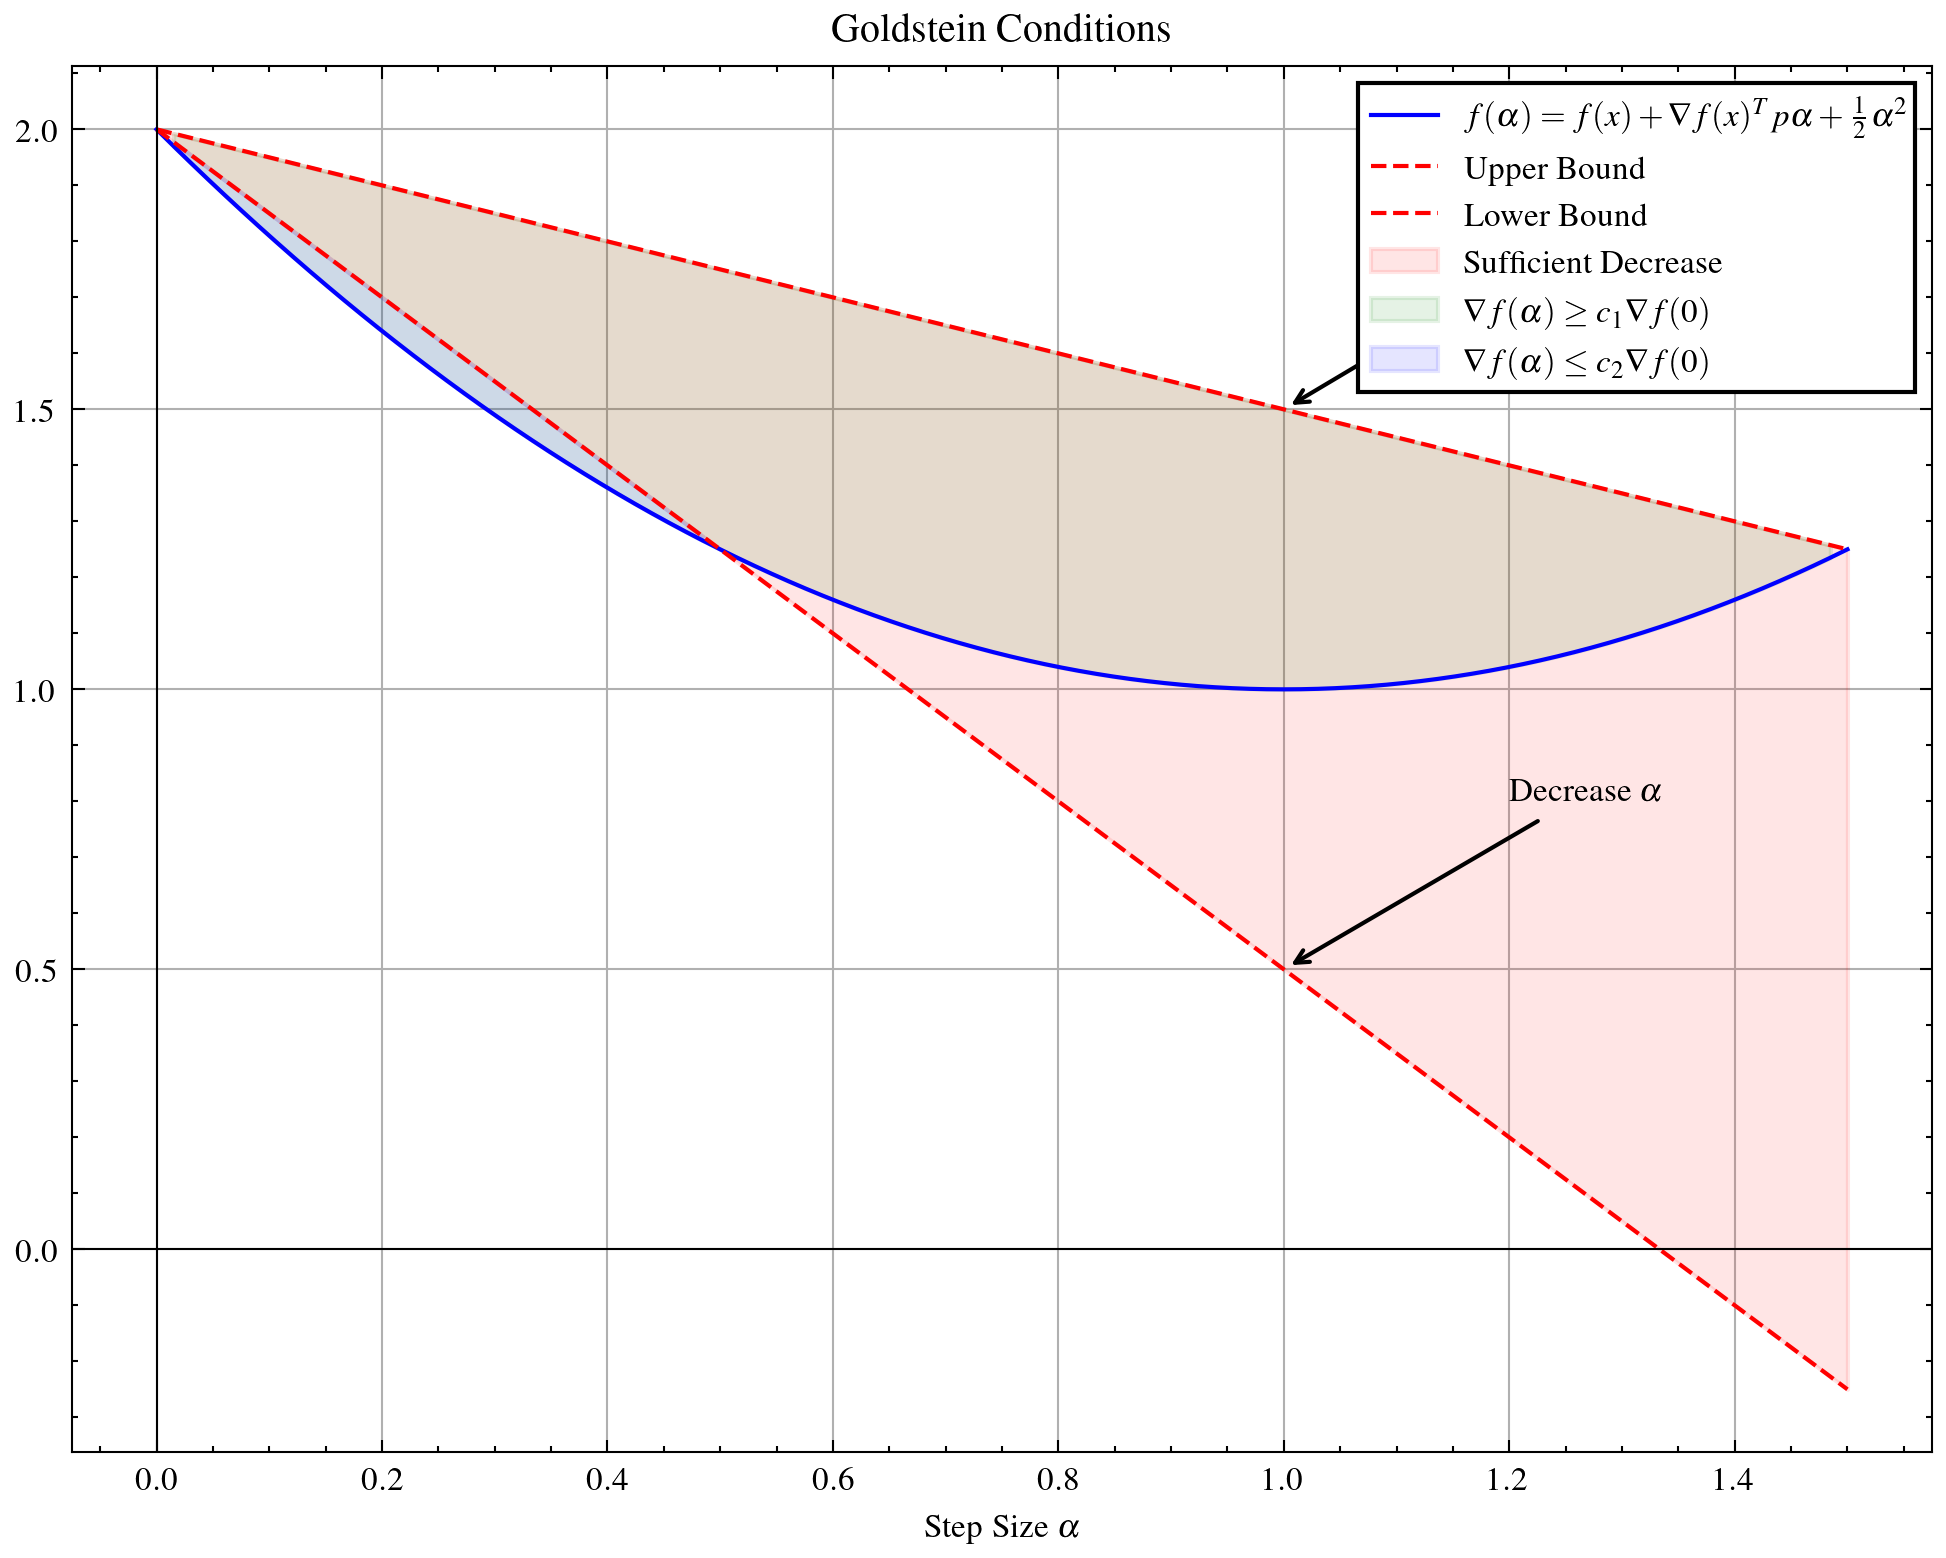
\includegraphics[width=0.8\textwidth]{figures/goldstein_conditions.png}
	\caption{Goldstein-betingelsene}
	\label{fig:goldstein_conditions}
\end{figure}

Goldstein-betingelsene brukes ofte i Newtons metode og kan være lettere å implementere enn Wolfe-betingelsene i visse sammenhenger.

\subsubsection{Goldstein-Wolfe-betingelsene}
\label{subsubsec:goldstein_wolfe_conditions}
Goldstein-Wolfe-betingelsene er en kombinasjon av Goldstein- og Wolfe-betingelsene, og gir en mer robust tilnærming til linjesøk.
Disse betingelsene sikrer at steglengden \(\alpha\) gir tilstrekkelig reduksjon i objektfunksjonen, samtidig som den opprettholder en viss krumning.
\begin{definition}{Goldstein-Wolfe-betingelsene}{goldstein_wolfe_conditions}
	Goldstein-Wolfe-betingelsene krever at Armijo- og Goldstein-betingelsene begge er oppfylt:
	\begin{enumerate}
		\item Armijo-betingelsen:
		      \[
			      f(\symbf{x} + \alpha \symbf{d})
			      \;\le\;
			      f(\symbf{x})
			      \;+\;
			      c_1\,\alpha\,\nabla f(\symbf{x})^T \symbf{d}.
		      \]
		\item Goldstein-betingelsen:
		      \[
			      f(\symbf{x}) + (1-c)\,\alpha\,\nabla f(\symbf{x})^T \symbf{d}
			      \;\le\;
			      f(\symbf{x} + \alpha \symbf{d})
			      \;\le\;
			      f(\symbf{x}) + c\,\alpha\,\nabla f(\symbf{x})^T \symbf{d}.
		      \]
	\end{enumerate}
	Disse betingelsene sikrer at steglengden \(\alpha\) gir tilstrekkelig reduksjon i objektfunksjonen, samtidig som den opprettholder en viss krumning.
\end{definition}
\begin{figure}[H]
	\centering
	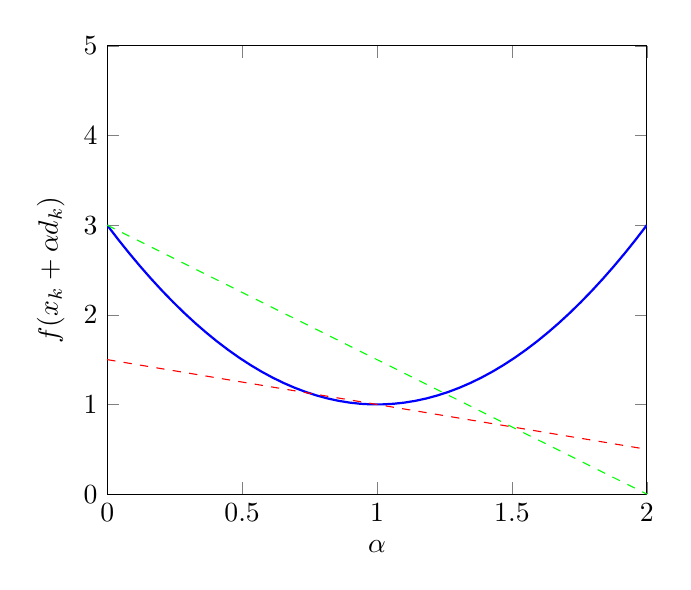
\begin{tikzpicture}
		\begin{axis}[
				xlabel={$\alpha$},
				ylabel={$f(\symbf{x}_k + \alpha \symbf{d}_k)$},
				xmin=0, xmax=2,
				ymin=0, ymax=5,
				samples=50,
				domain=0:2,
			]
			\addplot[blue, thick] {2*x^2 - 4*x + 3};
			\addplot[red, dashed] {1.5 - 0.5*x};
			\addplot[green, dashed] {3 - 1.5*x};
		\end{axis}
	\end{tikzpicture}
	\caption{Goldstein-Wolfe-betingelsene: Den blå kurven viser objektfunksjonen langs søkeretningen, mens den røde og grønne stiplede linjen viser de nedre og øvre grensene gitt av Goldstein-betingelsene. Alle steglengder $\alpha$ hvor den blå kurven ligger mellom de røde og grønne linjene er akseptable.}
	\label{fig:goldstein_wolfe_conditions}
\end{figure}


\subsection{Eksistens av gyldige steglengder}
\label{subsec:existence_step_length}

En viktig egenskap ved disse betingelsene er at det alltid eksisterer steglengder som oppfyller dem, gitt rimelige forutsetninger om objektfunksjonen:

\begin{theorem}{Eksistens av steglengder som tilfredsstiller betingelsene}{existence_step_length}
	La $f: \mathbb{R}^n \to \mathbb{R}$ være kontinuerlig deriverbar og la $\symbf{d}_k$ være en nedstigningsretning ved et punkt $\symbf{x}_k$. Anta at $f$ er nedenfra begrenset langs strålen $\{\symbf{x}_k + \alpha\symbf{d}_k : \alpha > 0\}$. Da eksisterer det intervaller av steglengder som tilfredsstiller både Armijo-, Wolfe- og Goldstein-betingelsene.
\end{theorem}

\begin{lemma}{Well-posedness av Wolfe-betingelsene}{well_posedness_wolfe_conditions}
	Anta at \(f:\R^n \to \R \) er kontinuerlig deriverbar. La \(\mathbf{p}_k\) være nedstigningsretningen ved iterasjon \(\mathbf{x}_k\), og anta at \(f\) er bundet nedenfra langs strålen:

	\[
		\{\mathbf{x}_k + \alpha \mathbf{p}_k : \alpha > 0\} \subset \mathbb{R}^n.
	\]

	Hvis \(0 < c_1 < c_2 < 1\), så eksisterer det intervaller av steglengder \(\alpha_k > 0\) slik at både Wolfe-betingelsene og Strong Wolfe-betingelsene er oppfylt.
\end{lemma}

\subsection{Konvergens av linjesøk-metoder}
\label{subsec:convergence_line_search}

Et sentralt resultat i optimeringsteori er at iterative algoritmer som bruker linjesøk med Wolfe-betingelsene konvergerer til stasjonære punkter under rimelige forutsetninger:

\begin{theorem}{Konvergens av linjesøk}{line_search_convergence}
	Anta at \(f\) er kontinuerlig deriverbar og at det finnes en \(\alpha^\ast > 0\) slik at
	\[
		f(\symbf{x} + \alpha^\ast \symbf{d}) < f(\symbf{x}) + \beta\,\alpha^\ast\,\nabla f(\symbf{x})^T \symbf{d}.
	\]
	Da vil Backtracking Line Search konvergere til en skrittlengde \(\alpha_k\) som tilfredsstiller Armijo-betingelsen.
\end{theorem}

Et mer generelt resultat er Zoutendijk's teorem:

\begin{theorem}{Zoutendijk's result}{zoutendijk_result}
	La \( \symbf{x}_{k+1} = \symbf{x}_k + \alpha_k \symbf{p}_k \), hvor \( \mathbf{p}_k \) er en nedstigningsretning, med skrittlengde \( \alpha_k \) som tilfredsstiller Wolfe-betingelsene.

	Anta at:
	\begin{itemize}
		\item \(f\) er bundet nedenfra i \(\R^n\)
		\item \(f\) er kontinuerlig deriverbar på det åpne settet \(\mathcal{N}\) som inneholder nivåsettet
		      \[ \mathcal{L} = \{\symbf{x}: f(\symbf{x}) \leq f(\symbf{x}_0)\} \]
		\item \(\nabla f\) er Lipschitz-kontinuerlig på \(\mathcal{N}\), dvs. det finnes en konstant \(L > 0\) slik at
		      \[ \|\nabla f(\symbf{x}) - \nabla f(\tilde{\symbf{x}})\| \leq L\|\symbf{x} - \tilde{\symbf{x}}\| \quad \text{for alle } \symbf{x}, \tilde{\symbf{x}} \in \mathcal{N} \]
	\end{itemize}

	Da har vi at:
	\[
		\sum_{k=0}^{\infty} \cos^2 \theta_k \| \nabla f(\symbf{x}_k) \|^2 < \infty,
	\]
	hvor \( \theta_k \) er vinkelen mellom \( \nabla f(\symbf{x}_k) \) og søkeretningen \( \symbf{p}_k \).

	Dette impliserer at \( \| \nabla f(\symbf{x}_k) \| \to 0 \) når \( k \to \infty \), som betyr at sekvensen av punkter konvergerer mot et stasjonært punkt.
\end{theorem}

Dette resultatet viser at optimeringsalgoritmer basert på linjesøk som tilfredsstiller Wolfe-betingelsene garanterer konvergens mot et stasjonært punkt, forutsatt at nivåsettet er begrenset og funksjonen oppfyller visse glatthetsegenskaper. Dette danner det teoretiske grunnlaget for mange praktiske optimeringsalgoritmer.

\subsection{Algoritmer for linjesøk}
\label{subsec:line_search_algorithms}

For å finne steglengder som tilfredsstiller disse betingelsene, er det utviklet flere praktiske algoritmer:

\subsubsection{Backtracking linjesøk}
\label{subsubsec:backtracking_line_search}
Backtracking linjesøk er en enkel og effektiv metode for å finne steglengder som tilfredsstiller Wolfe-betingelsene.
Den fungerer ved å starte med en initial steglengde \(\alpha_0 > 0\) og deretter redusere den til den tilfredsstiller betingelsene.
\footnote{For Newton, og Kvasi-Newton-metoder, er det vanlig å bruke \(\alpha_0 = 1\).}

\begin{algorithm}[H]
	\caption{Tilbakesporing linjesøk}
	\label{alg:backtracking_line_search}
	\KwIn{Initial steglengde \(\bar{\alpha} > 0\), reduksjonsfaktor \(\rho \in (0,1)\), Armijo-parameter \(c \in (0,1)\)}
	\KwOut{Steglengde \(\alpha_k\) som tilfredsstiller Armijo-betingelsen}
	\SetKwFunction{FMain}{BacktrackingLineSearch}
	\SetKwProg{Fn}{Function}{:}{}
	\Fn{\FMain{$\symbf{x}_k$, $\symbf{d}_k$}}{
		$\alpha \leftarrow \bar{\alpha}$ \;
		\Repeat{$f(\symbf{x}_k + \alpha \symbf{d}_k) \leq f(\symbf{x}_k) + c \alpha \nabla f(\symbf{x}_k)^T \symbf{d}_k$}{
			$\alpha \leftarrow \rho \cdot \alpha$ \;
		}
		\Return{$\alpha$}
	}
\end{algorithm}

\subsubsection{Zoom-algoritmen}
\label{subsubsec:zoom_algorithm}

For å finne steglengder som tilfredsstiller de sterke Wolfe-betingelsene, brukes ofte mer komplekse algoritmer som zoom-algoritmen:

\begin{algorithm}[H]
	\caption{Zoom-algoritme}
	\label{alg:zoom}
	\KwIn{Intervallgrenser $\alpha_{lo}$, $\alpha_{hi}$ som begrenser et område hvor Wolfe-betingelsene kan tilfredsstilles}
	\KwOut{Steglengde $\alpha_k$ som tilfredsstiller sterke Wolfe-betingelser}
	\While{konvergenskriterier ikke er oppfylt}{
		Interpolare $\alpha_j \in (\alpha_{lo}, \alpha_{hi})$ \;
		\eIf{$f(\symbf{x}_k + \alpha_j\symbf{d}_k) > f(\symbf{x}_k) + c_1\alpha_j\nabla f(\symbf{x}_k)^T\symbf{d}_k$ \textbf{eller} $f(\symbf{x}_k + \alpha_j\symbf{d}_k) \geq f(\symbf{x}_k + \alpha_{lo}\symbf{d}_k)$}{
			$\alpha_{hi} \leftarrow \alpha_j$ \tcc*{Reduser øvre grense}
		}{
			\eIf{$|\nabla f(\symbf{x}_k + \alpha_j\symbf{d}_k)^T\symbf{d}_k| \leq -c_2\nabla f(\symbf{x}_k)^T\symbf{d}_k$}{
				\Return{$\alpha_k = \alpha_j$}
			}{
				\eIf{$\nabla f(\symbf{x}_k + \alpha_j\symbf{d}_k)^T\symbf{d}_k \cdot ( \alpha_{hi} - \alpha_{lo}) \geq 0$}{
					$\alpha_{hi} \leftarrow \alpha_{lo}$
				}{}
				$\alpha_{lo} \leftarrow \alpha_j$ \tcc*{Oppdater nedre grense}
			}
		}
	}
\end{algorithm}

\chapter{Gradientfrie Optimeringsmetoder}
\label{sec:gradientfrie_metoder}

Gradientfrie metoder er optimeringsalgoritmer som ikke benytter gradienter eller Hesse-matriser i søket etter et minimum.
De egner seg spesielt godt i situasjoner der objektfunksjonen \( f : \mathbb{R}^n \to \mathbb{R} \) er:
\begin{itemize}
	\item ikke-differensierbar eller stykkevis glatt,
	\item støyete, simulert eller svartboksbasert,
	\item kostbar eller upraktisk å derivere.
\end{itemize}

I stedet for å bruke analytisk eller numerisk informasjon om deriverte, evaluerer slike metoder funksjonsverdier i ulike retninger eller punktkombinasjoner, og gjør fremskritt basert på hvilke punkter som gir forbedring.

Gradientfrie metoder kan være svært effektive når informasjonen om objektfunksjonen er begrenset. De gir imidlertid sjelden noen garanti for å finne et globalt minimum, eller for konvergens i klassisk forstand.

\subsection{Heuristiske metoder}

En heuristisk metode er en algoritme som forsøker å finne en god (men ikke nødvendigvis optimal) løsning ved å bruke forenklede regler, prøve-og-feile-strategier eller strategier inspirert av natur og erfaring.

De er spesielt utviklet for problemer der klassiske metoder feiler - for eksempel når funksjonen har mange lokale minima, er ikke-glatt, støyete eller kun tilgjengelig gjennom simulering.

\paragraph{Egenskaper ved heuristiske metoder}

\begin{itemize}
	\item Utfører ofte globalt søk (f.eks. gjennom tilfeldige steg eller populasjoner).
	\item Krever ikke deriverte eller Hessian.
	\item Har lav til moderat regnekostnad.
	\item Mangler garanti for optimalitet, men gir ofte svært gode løsninger i praksis.
\end{itemize}

\subsection{Nelder--Mead-algoritmen}
\label{sec:nelder_mead}

Nelder--Mead er en populær algoritme  for å minimere funksjoner uten å bruke gradienter eller Hesse-matriser.
Den er særlig nyttig når funksjonen er \emph{ikke-glatt}, \emph{støyete} eller \emph{utilgjengelig i lukket form}.

Algoritmen bruker et \textbf{simplex}~\ref{def:simplex} (et geometrisk objekt med \( n+1 \) hjørner i \( n \)-dimensjonalt rom) i \( \mathbb{R}^n \) for å iterativt søke mot et lokalt minimum.

\begin{minipage}[t]{0.56\textwidth}
	Metoden manipulerer simplexen ved hjelp av \textbf{4 operasjoner}:
	\noindent
	\begin{itemize}
		\item \emph{Refleksjon}: Speiler det dårligste punktet gjennom tyngdepunktet
		\item \emph{Ekspansjon}: Strekker simplekset i lovende retninger
		\item \emph{Kontraksjon}: Krymper simplekset når refleksjon ikke gir forbedring
		\item \emph{Krymping}: Reduserer hele simplekset mot beste punkt
	\end{itemize}
	Gjennom disse operasjonene tilpasser simplekset seg automatisk til funksjonens form og \enquote{Kryper} mot det lokale minimum uten behov for deriverte.
\end{minipage}
\hfill
\begin{minipage}[t]{0.40\textwidth}
	\begin{figure}[H]
		\centering
		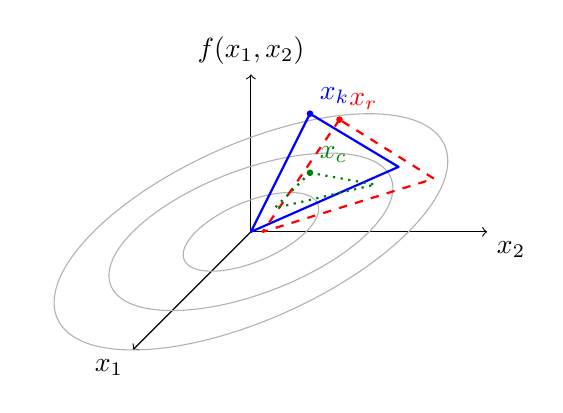
\begin{tikzpicture}[
				scale=1.0,
				x={(-0.5cm,-0.5cm)},
				y={(1cm,0cm)},
				z={(0cm,1cm)},
				line join=round
			]

			% Axes
			\draw[->] (0,0,0) -- (3,0,0) node[anchor=north east] {\( x_1 \)};
			\draw[->] (0,0,0) -- (0,3,0) node[anchor=north west] {\( x_2 \)};
			\draw[->] (0,0,0) -- (0,0,2) node[anchor=south] {\( f(x_1,x_2) \)};

			% Contours on base 
			\draw[black!30] (0,0,0) ellipse (3 and 2);
			\draw[black!30] (0,0,0) ellipse (2 and 1.5);
			\draw[black!30] (0,0,0) ellipse (1 and 0.7);

			% Initial simplex (blue solid) - scaled up by 1.5
			\draw[blue, thick]
			(1.5,1.5,2.25) -- (3,1.5,1.5) -- (2.25,3,1.95) -- cycle;

			% Reflected simplex (red dashed) - scaled up by 1.5
			\draw[red, thick, dashed]
			(0.75,1.5,1.8) -- (2.7,1.5,1.35) -- (1.65,3.15,1.5) -- cycle;

			% Contracted simplex (green dotted) - scaled up by 1.5
			\draw[green!50!black, thick, dotted]
			(1.8,1.65,1.65) -- (2.4,1.5,1.5) -- (1.95,2.55,1.575) -- cycle;

			% Key points only - scaled up by 1.5
			\fill[blue] (1.5,1.5,2.25) circle (1.2pt) node[above right] {\( x_k \)};
			\fill[red] (0.75,1.5,1.8) circle (1.2pt) node[above right] {\( x_r \)};
			\fill[green!50!black] (1.8,1.65,1.65) circle (1.2pt) node[above right] {\( x_c \)};

		\end{tikzpicture}
		\caption{Nelder-Mead algoritmen: Initialt (blå), reflektert (rød) og kontrahert (grønn) simplex med objektfunksjonens nivålinjer.}
		\label{fig:nelder_mead_3d}
	\end{figure}
\end{minipage}


\begin{algorithm}[H]
	\caption{Nelder--Mead-algoritme}
	\label{alg:nelder-mead}
	Initialiser simplex med \( n+1 \) punkter\;
	\Repeat{konvergenskriteriene er oppfylt}{
		Sorter simplex-punktene etter deres funksjonsverdi \( f(x_i) \)\;
		Beregn tyngdepunktet av de \( n \) beste punktene\;
		Reflekter det dårligste punktet gjennom tyngdepunktet for å få et nytt punkt \( x_r \)\;
		\uIf{\( f(x_1) \leq f(x_r) < f(x_n) \)}{
			Aksepter refleksjonen \( x_{n+1} \leftarrow x_r \)\;
		}
		\uElseIf{\( f(x_r) < f(x_1) \)}{
			Prøv ekspansjon til punkt \( x_e \)\;
			\If{\( f(x_e) < f(x_r) \)}{
				\( x_{n+1} \leftarrow x_e \)\;
			}
			\Else{
				\( x_{n+1} \leftarrow x_r \)\;
			}
		}
		\uElseIf{\( f(x_r) \geq f(x_n) \)}{
			Utfør en kontraksjon for å få punkt \( x_c \)\;
			\If{\( f(x_c) < f(x_{n+1}) \)}{
				\( x_{n+1} \leftarrow x_c \)\;
			}
			\Else{
				Krymp hele simplexet mot det beste punktet \( x_1 \)\;
			}
		}
	}
\end{algorithm}

\subsection{Andre gradientfrie metoder}

I tillegg til Nelder-Mead finnes det flere andre gradientfrie metoder:

\begin{itemize}
	\item \textbf{Genetiske algoritmer}: Inspirert av naturlig seleksjon, bruker populasjoner av løsninger som "evolusjonerer" over generasjoner.
	\item \textbf{Partikkelsverm-optimalisering (PSO)}: Inspirert av sosial atferd i fugleflokker eller fiskestimer, hvor partikler beveger seg i søkerommet.
	\item \textbf{Simulert annealing}: Inspirert av metallets varmebehandling, tillater algoritmen å akseptere dårligere løsninger med en viss sannsynlighet for å unngå å bli fanget i lokale minima.
\end{itemize}

\chapter{Førsteordens Optimeringsmetoder}
\label{chap:first_order_methods}

Førsteordens optimeringsmetoder bruker kun informasjon om objektfunksjonens gradient (første deriverte) for å finne minimumspunkter. Disse metodene er typisk enklere å implementere og krever mindre beregningskraft per iterasjon sammenlignet med andreordens metoder, noe som gjør dem egnet for store optimeringsproblemer.

\section{Gradientbaserte metoder}
\label{sec:gradient_based_methods}

Gradientbaserte metoder er en fundamental klasse av algoritmer hvor søkeretningen bestemmes direkte av gradienten til objektfunksjonen. Disse metodene er særlig nyttige når funksjonen er differensierbar, og når beregningskostnaden for å evaluere gradienten er akseptabel.

\subsection{Bratteste-nedstigning (Steepest descent)}

Bratteste-nedstigning, eller steepest descent, er den mest grunnleggende gradientbaserte optimeringsmetoden. Ideen er enkel: Følg retningen hvor funksjonen avtar raskest lokalt.

\begin{definition}{Steepest Descent}{steepest_descent}
	Steepest Descent-algoritmen oppdaterer iterasjonen \( \symbf{x}_k \) ved å ta et skritt i retning av den negative gradienten:
	\[
		\symbf{x}_{k+1} = \symbf{x}_k + \alpha_k \symbf{d}_k,
	\]
	hvor \( \alpha_k > 0 \) er skrittlengden og \( \symbf{d}_k = -\nabla f(\symbf{x}_k) \) er nedstigningsretningen.
\end{definition}

Søkeretningen er gitt ved:
\begin{equation}
	\symbf{d}_k = -\nabla f(\symbf{x}_k),
\end{equation}
som representerer retningen av bratteste nedstigning ved punktet \(\symbf{x}_k\).

\begin{algorithm}[H]
	\SetAlgoLined
	\KwIn{Startpunkt \( \symbf{x}_0 \), toleranse \( \epsilon \), maks antall iterasjoner \( K \)}
	\KwOut{Omtrentelig løsning \( \symbf{x}^\ast \)}
	\For{\( k = 0, 1, 2, \ldots, K\)}{
		\(\symbf{d}_k = -\nabla f(\symbf{x}_k)\)\;
		Finn skrittlengde \(\alpha_k\) (f.eks. ved linjesøk-metode)\;
		\(\symbf{x}_{k+1} = \symbf{x}_k + \alpha_k \symbf{d}_k\)\;
		\If{\(\|\nabla f(\symbf{x}_{k+1})\| < \epsilon\)}{
			\Return \(\symbf{x}_{k+1}\)\;
		}
	}
	\caption{Steepest Descent}
	\label{alg:steepest_descent}
\end{algorithm}

\subsubsection{Gradient Descent}
Gradient Descent er en spesialisert form for steepest descent som fokuserer på å minimere objektfunksjonen \(f\) ved å iterere over gradienten. Den er spesielt nyttig i maskinlæring og statistikk, hvor gradienten kan være kostbar å beregne.
\begin{definition}{Gradient Descent}{gradient_descent}
	Gradient Descent-algoritmen oppdaterer iterasjonen \( \symbf{x}_k \) ved å ta et skritt i retning av den negative gradienten:
	\[
		\symbf{x}_{k+1} = \symbf{x}_k - \alpha_k \nabla f(\symbf{x}_k),
	\]
	hvor \( \alpha_k > 0 \) er skrittlengden.
\end{definition}
\begin{algorithm}[H]
	\SetAlgoLined
	\KwIn{Startpunkt \( \symbf{x}_0 \), toleranse \( \epsilon \), maks antall iterasjoner \( K \)}
	\KwOut{Omtrentelig løsning \( \symbf{x}^\ast \)}
	\For{\( k = 0, 1, 2, \ldots, K\)}{
		Finn skrittlengde \(\alpha_k\) (f.eks. ved linjesøk-metode)\;
		\(\symbf{x}_{k+1} = \symbf{x}_k - \alpha_k \nabla f(\symbf{x}_k)\)\;
		\If{\(\|\nabla f(\symbf{x}_{k+1})\| < \epsilon\)}{
			\Return \(\symbf{x}_{k+1}\)\;
		}
	}
	\caption{Gradient Descent}
	\label{alg:gradient_descent}
\end{algorithm}

\subsection{Gradient Descent med Linjesøk}
\label{subsec:gd_line_search_variants}

Valget av linjesøkmetode har stor innflytelse på ytelsen til gradientbaserte algoritmer. Her presenterer vi gradient descent med ulike linjesøkstrategier.

\subsubsection{Gradient Descent with Exact Line Search}
\label{subsubsec:gd_exact_line_search}

Eksakt linjesøk finner den optimale steglengden i hver iterasjon:

\begin{algorithm}[H]
	\caption{Gradient Descent med Eksakt Linjesøk}
	\KwIn{Startpunkt \( \symbf{x}_0 \), toleranse \( \epsilon \)}
	\KwOut{Omtrentlig løsning \( \symbf{x}^\ast \)}
	\For{\( k = 0, 1, 2, \ldots\)}{
		\If{\(\|\nabla f(\symbf{x}_k)\| < \epsilon\)}{\Return \(\symbf{x}_k\)}
		\(\symbf{d}_k = -\nabla f(\symbf{x}_k)\)\;
		\(\alpha_k = \arg\min_{\alpha > 0} f(\symbf{x}_k + \alpha \symbf{d}_k)\)\;
		\(\symbf{x}_{k+1} = \symbf{x}_k + \alpha_k \symbf{d}_k\)\;
	}
\end{algorithm}

Dette er teoretisk optimalt, men eksakt linjesøk er sjelden praktisk gjennomførbart for komplekse funksjoner.

\subsubsection{Gradient Descent with Backtracking Line Search}
\label{subsubsec:gd_backtracking}

Backtracking linjesøk er en praktisk og effektiv tilnærming som baserer seg på Armijo-betingelsen:

\begin{algorithm}[H]
	\caption{Gradient Descent med Backtracking Linjesøk}
	\KwIn{Startpunkt \( \symbf{x}_0 \), toleranse \( \epsilon \), parametre \( c \in (0,1) \), \( \rho \in (0,1) \)}
	\KwOut{Omtrentlig løsning \( \symbf{x}^\ast \)}
	\For{\( k = 0, 1, 2, \ldots\)}{
		\If{\(\|\nabla f(\symbf{x}_k)\| < \epsilon\)}{\Return \(\symbf{x}_k\)}
		\(\symbf{d}_k = -\nabla f(\symbf{x}_k)\)\;
		\(\alpha = 1\) \tcc*{Initial steglengde}
		\While{$f(\symbf{x}_k + \alpha \symbf{d}_k) > f(\symbf{x}_k) + c\,\alpha\,\nabla f(\symbf{x}_k)^T \symbf{d}_k$}{
			\(\alpha = \rho \cdot \alpha\) \tcc*{Reduser steglengden}
		}
		\(\symbf{x}_{k+1} = \symbf{x}_k + \alpha \symbf{d}_k\)\;
	}
\end{algorithm}

Denne metoden er mye brukt i praksis på grunn av sin enkelhet og effektivitet.

\subsubsection{Gradient Descent with Wolfe Line Search}
\label{subsubsec:gd_wolfe}

Wolfe linjesøk sikrer både tilstrekkelig reduksjon og at steget ikke er for kort:

\begin{algorithm}[H]
	\caption{Gradient Descent med Wolfe Linjesøk}
	\KwIn{Startpunkt \( \symbf{x}_0 \), toleranse \( \epsilon \), parametre \( c_1, c_2 \in (0,1) \) med \( c_1 < c_2 \)}
	\KwOut{Omtrentlig løsning \( \symbf{x}^\ast \)}
	\For{\( k = 0, 1, 2, \ldots\)}{
		\If{\(\|\nabla f(\symbf{x}_k)\| < \epsilon\)}{\Return \(\symbf{x}_k\)}
		\(\symbf{d}_k = -\nabla f(\symbf{x}_k)\)\;
		\(\alpha_{\text{lo}} = 0\); \(\alpha_{\text{hi}} = +\infty\); \(\alpha = 1\)\;
		\(\phi_0 = f(\symbf{x}_k)\); \(\phi_0' = \nabla f(\symbf{x}_k)^T \symbf{d}_k\) \;
		\While{true}{
			\(\phi_\alpha = f(\symbf{x}_k + \alpha \symbf{d}_k)\); \(\phi_\alpha' = \nabla f(\symbf{x}_k + \alpha \symbf{d}_k)^T \symbf{d}_k\) \;
			\If{\(\phi_\alpha > \phi_0 + c_1 \alpha \phi_0'\) \textbf{or} \((\phi_\alpha \geq \phi_{\alpha_{\text{lo}}} \text{ and } \alpha > \alpha_{\text{lo}})\)}{
				\(\alpha_{\text{hi}} = \alpha\); \(\alpha = \frac{\alpha_{\text{lo}} + \alpha_{\text{hi}}}{2}\); \textbf{continue}\;
			}
			\If{\(|\phi_\alpha'| \leq -c_2 \phi_0'\)}{\textbf{break}}
			\If{\(\phi_\alpha' \geq 0\)}{
				\(\alpha_{\text{hi}} = \alpha_{\text{lo}}\); \(\alpha_{\text{lo}} = \alpha\); \(\alpha = \frac{\alpha_{\text{lo}} + \alpha_{\text{hi}}}{2}\)\;
			}
			\Else{
				\(\alpha_{\text{lo}} = \alpha\);
				\(\alpha = \)(\(\alpha_{\text{hi}} < +\infty\)) ? \(\frac{\alpha_{\text{lo}} + \alpha_{\text{hi}}}{2}\) : \(2\alpha_{\text{lo}}\)\;
			}
		}
		\(\symbf{x}_{k+1} = \symbf{x}_k + \alpha \symbf{d}_k\)\;
	}
\end{algorithm}

Wolfe linjesøk er spesielt viktig for kvasi-Newton-metoder, men forbedrer også ytelsen til gradient descent.

\subsubsection{Gradient Descent with Strong Wolfe Line Search}
\label{subsubsec:gd_strong_wolfe}

Strong Wolfe linjesøk legger til en ytterligere begrensning på absoluttverdi:

\begin{algorithm}[H]
	\caption{Gradient Descent med Strong Wolfe Linjesøk}
	\KwIn{Startpunkt \( \symbf{x}_0 \), toleranse \( \epsilon \), parametre \( c_1, c_2 \)}
	\KwOut{Omtrentlig løsning \( \symbf{x}^\ast \)}
	\For{\( k = 0, 1, 2, \ldots\)}{
		\If{\(\|\nabla f(\symbf{x}_k)\| < \epsilon\)}{\Return \(\symbf{x}_k\)}
		\(\symbf{d}_k = -\nabla f(\symbf{x}_k)\)\;
		\(\alpha_{\text{lo}} = 0\); \(\alpha_{\text{hi}} = +\infty\); \(\alpha = 1\)\;
		\(\phi_0 = f(\symbf{x}_k)\); \(\phi_0' = \nabla f(\symbf{x}_k)^T \symbf{d}_k\) \;
		\While{true}{
			\(\phi_\alpha = f(\symbf{x}_k + \alpha \symbf{d}_k)\); \(\phi_\alpha' = \nabla f(\symbf{x}_k + \alpha \symbf{d}_k)^T \symbf{d}_k\) \;
			\If{\(\phi_\alpha > \phi_0 + c_1 \alpha \phi_0'\) \textbf{or} \((\phi_\alpha \geq \phi_{\alpha_{\text{lo}}}\)}{
				\(\alpha_{\text{hi}} = \alpha\); \(\alpha = \frac{\alpha_{\text{lo}} + \alpha_{\text{hi}}}{2}\); \textbf{continue}\;
			}
			\If{\(|\phi_\alpha'| \leq c_2 |\phi_0'|\)}{\textbf{break}}
			\If{\(\phi_\alpha' \cdot (\alpha_{\text{hi}} - \alpha_{\text{lo}}) \geq 0\)}{\(\alpha_{\text{hi}} = \alpha_{\text{lo}}\)}
			\(\alpha_{\text{lo}} = \alpha\);
			\(\alpha = (\alpha_{\text{hi}} < +\infty\)) ? \(\frac{\alpha_{\text{lo}} + \alpha_{\text{hi}}}{2}\) : \(2\alpha_{\text{lo}}\)\;
		}
		\(\symbf{x}_{k+1} = \symbf{x}_k + \alpha \symbf{d}_k\)\;
	}
\end{algorithm}

Dette er særlig nyttig for algoritmer som konjugert gradient der kontroll over oscillering er viktig.

\subsubsection{Gradient Descent with Goldstein Line Search}
\label{subsubsec:gd_goldstein}

Goldstein linjesøk sikrer at steglengden er innenfor et bestemt intervall:

\begin{algorithm}[H]
	\caption{Gradient Descent med Goldstein Linjesøk}
	\KwIn{Startpunkt \( \symbf{x}_0 \), toleranse \( \epsilon \), parameter \( c \in (0,0.5) \)}
	\KwOut{Omtrentlig løsning \( \symbf{x}^\ast \)}
	\For{\( k = 0, 1, 2, \ldots\)}{
		\If{\(\|\nabla f(\symbf{x}_k)\| < \epsilon\)}{\Return \(\symbf{x}_k\)}
		\(\symbf{d}_k = -\nabla f(\symbf{x}_k)\)\;
		\(\alpha_{\text{min}} = 0\); \(\alpha_{\text{max}} = +\infty\); \(\alpha = 1\)\;
		\(\phi_0 = f(\symbf{x}_k)\); \(\phi_0' = \nabla f(\symbf{x}_k)^T \symbf{d}_k\) \;
		\While{true}{
			\(\phi_\alpha = f(\symbf{x}_k + \alpha \symbf{d}_k)\) \;
			\If{\(\phi_\alpha > \phi_0 + c \cdot \alpha \cdot \phi_0'\)}{
				\(\alpha_{\text{max}} = \alpha\); \(\alpha = \frac{\alpha_{\text{min}} + \alpha_{\text{max}}}{2}\); \textbf{continue}\;
			}
			\If{\(\phi_\alpha < \phi_0 + (1-c) \cdot \alpha \cdot \phi_0'\)}{
				\(\alpha_{\text{min}} = \alpha\);
				\(\alpha = \)(\(\alpha_{\text{max}} < +\infty\)) ? \(\frac{\alpha_{\text{min}} + \alpha_{\text{max}}}{2}\) : \(2\alpha\);
				\textbf{continue}\;
			}
			\textbf{break} \tcc*{Goldstein-betingelser oppfylt}
		}
		\(\symbf{x}_{k+1} = \symbf{x}_k + \alpha \symbf{d}_k\)\;
	}
\end{algorithm}

Goldstein betingelsene danner effektivt et "bånd" rundt den lineære approksimasjonen av funksjonen.

\subsubsection{Sammenligning av linjesøkmetoder}
\label{subsubsec:line_search_comparison}

Valg av linjesøkmetode påvirker ytelsen til gradient descent på flere måter:

\begin{table}[H]
	\centering
	\begin{tabular}{|l|c|c|c|}
		\hline
		\textbf{Linjesøkmetode} & \textbf{Beregningskostnad} & \textbf{Robusthet} & \textbf{Egnet for}                      \\
		\hline
		Eksakt                  & Høy                        & Moderat            & Enkle funksjoner, kvadratiske problemer \\
		\hline
		Backtracking            & Lav                        & God                & Generelle problemer, rask prototyping   \\
		\hline
		Wolfe                   & Middels                    & Meget god          & Kvasi-Newton metoder                    \\
		\hline
		Strong Wolfe            & Middels-høy                & Meget god          & Konjugerte gradient metoder             \\
		\hline
		Goldstein               & Middels                    & God                & Newton-baserte metoder                  \\
		\hline
	\end{tabular}
	\caption{Sammenligning av linjesøkmetoder for gradient descent}
	\label{tab:line_search_comparison}
\end{table}

I praksis er backtracking linjesøk ofte førstevalget på grunn av sin enkelhet og effektivitet, mens Wolfe-betingelsene er foretrukket for mer sofistikerte algoritmer som krever mer nøyaktige steglengder for optimal konvergens.

\subsection{Konvergensanalyse og begrensninger}
\label{subsec:steepest_descent_convergence}

For å forstå konvergensen av Steepest Descent, betrakter vi først det ideelle tilfellet hvor objektfunksjonen er kvadratisk med en positiv definit og symmetrisk Hesse-matrise \(Q\):

\begin{align*}
	f(\symbf{x})        & = \frac{1}{2} \symbf{x}^T Q \symbf{x} - \symbf{b}^T \symbf{x} + c \\
	\nabla f(\symbf{x}) & = Q \symbf{x} - \symbf{b}
\end{align*}

For denne kvadratiske funksjonen er det optimale punktet \(\symbf{x}^\ast\) løsningen av ligningen \(Q \symbf{x}^\ast = \symbf{b}\).

Med eksakt linjesøk kan vi finne den optimale steglengden \(\alpha_k\) som gitt ved:

\[
	\alpha_k = \frac{\nabla f_k^\top \nabla f_k}{\nabla f_k^\top Q \nabla f_k}
\]

Dette gir oppdateringen:
\begin{equation}
	\symbf{x}_{k+1} = \symbf{x}_k - \frac{\nabla f_k^\top \nabla f_k}{\nabla f_k^\top Q \nabla f_k} \nabla f_k
\end{equation}

\begin{theorem}{Konvergenshastighet for Steepest Descent}{steepest_descent_convergence}
	Når Steepest Descent-metoden med eksakte linjesøk anvendes på en sterkt konveks kvadratisk funksjon, er konvergenshastigheten begrenset av:
	\[
		\norm{\symbf{x}_{k+1} - \symbf{x}^\ast}_Q^2 \leq \left(\frac{\kappa - 1}{\kappa + 1}\right)^2 \norm{\symbf{x}_k - \symbf{x}^\ast}_Q^2,
	\]
	hvor \( \kappa = \frac{\lambda_n}{\lambda_1} \) er kondisjonstallet til \( Q \), med \( 0 < \lambda_1 \leq \lambda_2 \leq \cdots \leq \lambda_n \) som egenverdiene til \( Q \).
\end{theorem}

Dette resultatet viser at konvergenshastigheten til Steepest Descent er sterkt påvirket av kondisjonstallet \( \kappa \). For dårlig kondisjonerte problemer (høy \(\kappa\)), vil faktoren \( \frac{\kappa - 1}{\kappa + 1} \) nærme seg 1, noe som resulterer i ekstremt langsom konvergens.

\begin{theorem}{Asymptotisk konvergens av Steepest Descent}{steepest_descent_general}
	Anta at \(f : \mathbb{R}^n \to \mathbb{R}\) er to ganger kontinuerlig deriverbar og at iteratene \(\symbf{x}_k\) generert av Steepest Descent med eksakt linjesøk konvergerer til et punkt \(x^\ast\), hvor Hesse-matrisen \(\nabla^2 f(x^\ast)\) er positiv definit.

	La \(\lambda_1 \leq \lambda_2 \leq \cdots \leq \lambda_n\) være egenverdiene til \(\nabla^2 f(x^\ast)\). Da finnes det en konstant \(r \in \left( \frac{\lambda_n - \lambda_1}{\lambda_n + \lambda_1}, 1 \right)\) slik at
	\[
		f(x_{k+1}) - f(x^\ast) \leq r^2 \left[ f(x_k) - f(x^\ast) \right]
	\]
	for alle tilstrekkelig store \(k\).
\end{theorem}

Dette teoremet bekrefter at metoden har \emph{lineær konvergens}, men at konvergensfaktoren \(r^2\) blir nær 1 når kondisjonstallet \(\kappa = \lambda_n / \lambda_1\) er stort. I praksis betyr dette at steepest descent kan konvergere ekstremt langsomt for dårlig kondisjonerte problemer, selv under ideelle forhold.

Hovedbegrensningene ved steepest descent inkluderer:
\begin{itemize}
	\item Zigzag-konvergens på dårlig kondisjonerte problemer
	\item Lineær konvergensrate (som kan være svært langsom)
	\item Sensitivitet til skalering av variablene
\end{itemize}

\subsection{Momentumbaserte varianter}
\label{subsec:momentum_methods}

For å overkomme noen av begrensningene til steepest descent, har momentumbaserte varianter blitt utviklet. Disse metodene bruker informasjon fra tidligere iterasjoner for å akselerere konvergensen og redusere zigzag-bevegelsen.

\begin{definition}{Gradient Descent med Momentum}{momentum_gd}
	Gradient descent med momentum oppdaterer iterasjonen ved:
	\begin{align*}
		\symbf{v}_{k+1} & = \beta \symbf{v}_k + \alpha_k \nabla f(\symbf{x}_k) \\
		\symbf{x}_{k+1} & = \symbf{x}_k - \symbf{v}_{k+1}
	\end{align*}
	hvor \(\beta \in [0, 1)\) er momentumparameteren og \(\symbf{v}_k\) er momentumvektoren.
\end{definition}

Momentumteknikken akselererer konvergensen ved å:
\begin{itemize}
	\item Akkumulere "hastighet" i konsistente retninger
	\item Dempe oscillasjoner i inkonsekvente retninger
	\item Hjelpe algoritmen med å unnslippe flate regioner og små lokale minima
\end{itemize}

\begin{definition}{Nesterov Akselerert Gradient (NAG)}{nesterov_ag}
	Nesterov akselerert gradient er en videreutvikling av momentum hvor gradienten evalueres ved et predikert punkt:
	\begin{align*}
		\symbf{y}_k     & = \symbf{x}_k + \beta \symbf{v}_k                    \\
		\symbf{v}_{k+1} & = \beta \symbf{v}_k + \alpha_k \nabla f(\symbf{y}_k) \\
		\symbf{x}_{k+1} & = \symbf{x}_k - \symbf{v}_{k+1}
	\end{align*}
\end{definition}

Nesterov-akselerasjon forbedrer konvergensen ytterligere ved å ta en "forhåndsvisning" av neste punkt før beregning av gradienten, noe som gir en mer fremtidsrettet korrigering.

For konvekse problemer kan Nesterov akselerert gradient oppnå en konvergensrate på \(O(1/k^2)\) i funksjonsverdier, sammenlignet med \(O(1/k)\) for standard gradient descent, hvor \(k\) er antall iterasjoner.

\section{Konjugerte Gradientmetoder (CG)}
\label{sec:cg_methods}

\subsection{Motivasjon og utledning}
\label{subsec:cg_motivation}
Konjugerte gradientmetoder er en klasse av optimeringsalgoritmer som er spesielt utviklet for å løse store, tette (sparse) systemer av lineære ligninger og kvadratiske optimeringsproblemer. De er basert på ideen om å bruke gradientinformasjon til å konstruere en sekvens av konjugerte retninger, som reduserer antall nødvendige iterasjoner for å nå et minimum.
Disse metodene er spesielt nyttige når Hesse-matrisen er stor og sparsom, og de kan oppnå kvadratisk konvergens i antall iterasjoner.
\begin{definition}{Konjugerte gradientmetoder}{conjugate_gradient}
	Konjugerte gradientmetoder er iterative algoritmer for å løse systemer av lineære ligninger eller minimere kvadratiske funksjoner av formen:
	\[
		f(\symbf{x}) = \frac{1}{2} \symbf{x}^T A \symbf{x} - \symbf{b}^T \symbf{x}
	\]
	hvor \(A\) er en symmetrisk positiv definit matrise.
	Konjugerte gradientmetoder bruker gradientinformasjon til å konstruere en sekvens av konjugerte retninger \(\symbf{p}_k\) og oppdaterer løsningen iterativt:
	\[
		\symbf{x}_{k+1} = \symbf{x}_k + \alpha_k \symbf{p}_k
	\]
	hvor \(\alpha_k\) er skrittlengden bestemt av linjesøk.
\end{definition}

\begin{definition}{Konjugerte retninger}{conjugate_directions}
	To retninger \(\symbf{p}, \symbf{q}\) er konjugerte med hensyn til en matrise \(A\) hvis:
	\[
		\symbf{p}^T A \symbf{q} = 0
	\]
\end{definition}

Dette betyr at de er ortogonale i forhold til den indre produkt definert av \(A\). I konjugerte gradientmetoder brukes konjugerte retninger for å sikre at hver iterasjon er uavhengig av de tidligere iterasjonene.
\begin{itemize}
	\item \(\symbf{p}_k^T A \symbf{p}_j = 0\) for \(k \neq j\)
	\item \(\symbf{p}_k^T A \symbf{p}_k > 0\) for alle \(k\)
\end{itemize}
Dette sikrer at hver ny retning er konjugert med hensyn til de tidligere retningene, noe som reduserer antall nødvendige iterasjoner for å nå et minimum.

\begin{example}{Konjugerte gradientmetoder}{cg_example}
	Anta at vi har en kvadratisk funksjon \(f(\symbf{x})\) med Hesse-matrise \(A\). Ved å bruke konjugerte gradientmetoder kan vi iterativt oppdatere løsningen \(\symbf{x}_k\) ved å velge konjugerte retninger \(\symbf{p}_k\) og bestemme skrittlengden \(\alpha_k\) ved linjesøk.
	\[
		\symbf{x}_{k+1} = \symbf{x}_k + \alpha_k \symbf{p}_k
	\]

	Den første retningen \(\symbf{p}_0\) er valgt som den negative gradienten \(-\nabla f(\symbf{x}_0)\), og den andre retningen \(\symbf{p}_1\) er konjugert til \(\symbf{p}_0\) med hensyn til Hesse-matrisen \(A\).
	\[
		\symbf{p}_1 = -\nabla f(\symbf{x}_1) + \beta_1 \symbf{p}_0
	\]
	Deretter oppdateres løsningen \(\symbf{x}_1\) ved å bruke den første retningen \(\symbf{p}_0\), og den andre retningen \(\symbf{p}_1\) brukes til å oppdatere løsningen \(\symbf{x}_2\).

	Vi gjentar dette til konvergenskriteriene er oppfylt, dvs. når gradienten \(\nabla f(\symbf{x}_k)\) er tilstrekkelig liten.
	\[
		\|\nabla f(\symbf{x}_k)\| \approx 0
	\]

	\begin{figure}[H]
		\centering
		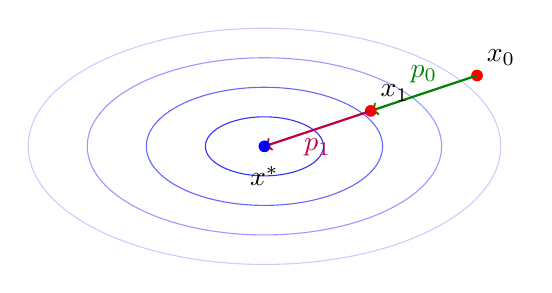
\begin{tikzpicture}[scale=1.5]
			% Contour plot av en elliptisk kvadratisk funksjon
			\draw[blue!20] (0,0) ellipse (2 and 1);
			\draw[blue!40] (0,0) ellipse (1.5 and 0.75);
			\draw[blue!60] (0,0) ellipse (1 and 0.5);
			\draw[blue!80] (0,0) ellipse (0.5 and 0.25);

			% Startpunktet
			\node[circle, fill=red, inner sep=1.5pt] (x0) at (1.8,0.6) {};
			\node[above right] at (x0) {$\symbf{x}_0$};

			% Første gradient og retning
			\draw[->, thick, green!50!black] (1.8,0.6) -- (0.9,0.3) node[midway, above] {$\symbf{p}_0$};

			% Første iterasjon
			\node[circle, fill=red, inner sep=1.5pt] (x1) at (0.9,0.3) {};
			\node[above right] at (x1) {$\symbf{x}_1$};

			% Andre retning (konjugert til første)
			\draw[->, thick, purple] (0.9,0.3) -- (0,0) node[midway, below] {$\symbf{p}_1$};

			% Minimum
			\node[circle, fill=blue, inner sep=1.5pt] at (0,0) {};
			\node at (0,-0.25) {$\symbf{x}^*$};
		\end{tikzpicture}
		\caption{Konjugerte gradientmetoder: Konturplot av en kvadratisk funksjon med konjugerte retninger. Merk hvordan den første retningen $\symbf{p}_0$ følger den negative gradienten, mens den andre retningen $\symbf{p}_1$ er konjugert til $\symbf{p}_0$ og leder direkte til minimumet.}
		\label{fig:cg_example}
	\end{figure}

	I dette eksempelet når algoritmen minimumet på bare to iterasjoner fordi retningene er konjugerte med hensyn på Hesse-matrisen. For en kvadratisk funksjon i $n$ dimensjoner vil konjugert gradient konvergere i maksimalt $n$ iterasjoner.

\end{example}

\subsection{Ikke-lineære Konjugerte Gradientmetoder}
For generelle ikke-lineære funksjoner tilpasses CG-metoden ved å oppdatere søkeretningen basert på den nåværende gradienten og tidligere søkeretninger. De to mest kjente variantene er Fletcher-Reeves (FR) og Polak-Ribière (PR).

\begin{algorithm}[H]
	\SetAlgoLined
	\KwIn{Startpunkt \(\symbf{x}_0\), toleranse \(\epsilon > 0\)}
	\KwOut{Omtrentelig løsning \(\symbf{x}^\ast\)}
	\(\symbf{g}_0 \gets \nabla f(\symbf{x}_0)\) \tcc*{Gradient}
	\(\symbf{p}_0 \gets -\symbf{g}_0\) \tcc*{Første søkeretning}
	\For{\(k = 0, 1, 2, \ldots\)}{
		\If{\(\|\symbf{g}_k\| < \epsilon\)}{
			\Return \(\symbf{x}_k\) \tcc*{Konvergens oppnådd}
		}
		Finn \(\alpha_k\) ved linjesøk som minimerer \(f(\symbf{x}_k + \alpha\symbf{p}_k)\) \;
		\(\symbf{x}_{k+1} \gets \symbf{x}_k + \alpha_k\symbf{p}_k\) \tcc*{Oppdater løsning}
		\(\symbf{g}_{k+1} \gets \nabla f(\symbf{x}_{k+1})\) \tcc*{Ny gradient}
		Beregn \(\beta_{k+1}\) \tcc*{FR eller PR formel}
		\(\symbf{p}_{k+1} \gets -\symbf{g}_{k+1} + \beta_{k+1}\symbf{p}_k\) \tcc*{Ny søkeretning}
	}
	\caption{Ikke-lineær Konjugert Gradient Metode}
\end{algorithm}

Valget av \(\beta_{k+1}\) er avgjørende for metodens ytelse:
\begin{definition}{Gradient og søkeretning}{gradient_direction}
	I konjugerte gradientmetoder er:
	\begin{itemize}
		\item \(\symbf{g}_k = \nabla f(\symbf{x}_k)\) gradienten ved punkt \(\symbf{x}_k\)
		\item \(\symbf{p}_k\) søkeretningen ved iterasjon \(k\)
	\end{itemize}
\end{definition}

\begin{definition}{Fletcher-Reeves koeffisient}{fletcher_reeves}
	Fletcher-Reeves koeffisienten for konjugerte gradientmetoder er definert som:
	\[
		\beta_{k+1}^{FR} = \frac{\symbf{g}_{k+1}^T\symbf{g}_{k+1}}{\symbf{g}_k^T\symbf{g}_k}
	\]
	Dette er forholdet mellom kvadratet av normen til den nåværende og forrige gradienten.
\end{definition}

\begin{definition}{Polak-Ribière koeffisient}{polak_ribiere}
	Polak-Ribière koeffisienten for konjugerte gradientmetoder er definert som:
	\[
		\beta_{k+1}^{PR} = \frac{\symbf{g}_{k+1}^T(\symbf{g}_{k+1} - \symbf{g}_k)}{\symbf{g}_k^T\symbf{g}_k}
	\]
	Denne formelen måler endringen i gradienten relativt til den forrige gradienten.
\end{definition}

\begin{definition}{Hestenes-Stiefel koeffisient}{hestenes_stiefel}
	Hestenes-Stiefel koeffisienten for konjugerte gradientmetoder er definert som:
	\[
		\beta_{k+1}^{HS} = \frac{\symbf{g}_{k+1}^T(\symbf{g}_{k+1} - \symbf{g}_k)}{\symbf{p}_k^T(\symbf{g}_{k+1} - \symbf{g}_k)}
	\]
	Denne formelen tar hensyn til både gradientendringen og forrige søkeretning.
\end{definition}

Polak-Ribière-metoden har ofte bedre ytelse i praksis og har egenskapen at når \(\beta_{k+1}^{PR} < 0\), kan det være fordelaktig å sette \(\beta_{k+1}^{PR} = 0\), noe som effektivt gjør en omstart av algoritmen ved å ta et steepest descent-steg.

\begin{corollary}{Broydens metode}{broydens_method}
	Broydens metode er en variant av konjugert gradientmetoden som bruker en sekvens av gradientretninger og oppdaterer Hesse-matrisen ved hjelp av BFGS-formelen. Den er spesielt nyttig for ikke-lineære problemer hvor Hesse-matrisen ikke er lett tilgjengelig.
	\[
		\symbf{B}_{k+1} = \symbf{B}_k + \frac{(\symbf{y}_k - \symbf{B}_k\symbf{s}_k)(\symbf{y}_k - \symbf{B}_k\symbf{s}_k)^T}{(\symbf{s}_k^T \symbf{y}_k)}
	\]
	hvor \(\symbf{y}_k = \nabla f(\symbf{x}_{k+1}) - \nabla f(\symbf{x}_k)\) og \(\symbf{s}_k = \symbf{x}_{k+1} - \symbf{x}_k\).
\end{corollary}

\subsection{Prekondisjoneringstekniker}
\label{subsec:cg_preconditioning}

For dårlig kondisjonerte problemer kan konvergensen til konjugert gradient-metoden forbedres betydelig gjennom prekondisjonering. Ideen er å transformere det originale problemet til et som har et bedre kondisjonstall.

\begin{definition}{Prekondisjonert konjugert gradient}{preconditioned_cg}
	La \(M\) være en symmetrisk positiv definit matrise som approksimerer \(A\) på en måte som gjør at systemet \(Mz = r\) er lett å løse. Den prekondisjonerte konjugerte gradient-metoden løser det transformerte systemet:
	\[
		M^{-1}A\symbf{x} = M^{-1}\symbf{b}
	\]
\end{definition}

Gode prekondisjonerere reduserer kondisjonstallet \(\kappa(M^{-1}A)\) sammenlignet med \(\kappa(A)\), og dette resulterer i raskere konvergens.

Vanlige prekondisjoneringsteknikker inkluderer:
\begin{itemize}
	\item Jacobi-prekondisjonering (diagonal skalering)
	\item Ufullstendig Cholesky-faktorisering
	\item Ufullstendig LU-faktorisering
	\item Algebraiske multigrid-metoder
\end{itemize}

\subsection{Konvergensegenskaper}
\label{subsec:cg_convergence}

For lineære systemer med en symmetrisk positiv definit matrise \(A\) har konjugert gradient-metoden følgende konvergensegenskaper:

\begin{theorem}{CG-konvergens}{cg_convergence}
	La \(A\) være en symmetrisk positiv definit matrise med egenverdier \(\lambda_1 \leq \lambda_2 \leq \cdots \leq \lambda_n\). Den konjugerte gradient-metoden gir iterasjoner \(\symbf{x}_k\) som tilfredsstiller:
	\[
		\|\symbf{x}_k - \symbf{x}^*\|_A \leq 2 \left(\frac{\sqrt{\kappa} - 1}{\sqrt{\kappa} + 1}\right)^k \|\symbf{x}_0 - \symbf{x}^*\|_A
	\]
	hvor \(\kappa = \lambda_n/\lambda_1\) er kondisjonstallet til \(A\) og \(\|\symbf{v}\|_A = \sqrt{\symbf{v}^T A \symbf{v}}\).
\end{theorem}

Dette viser at konvergenshastigheten er avhengig av kvadratroten av kondisjonstallet, noe som er bedre enn for steepest descent. I tillegg garanterer konjugert gradient-metoden eksakt konvergens etter maksimalt \(n\) iterasjoner i eksakt aritmetikk, hvor \(n\) er dimensjonen til problemet.

For ikke-lineære problemer er konvergensanalysen mer komplisert, men under visse antagelser kan ikke-lineær konjugert gradient med periodiske omstarter oppnå lineær konvergenshastighet:

\begin{theorem}{Konvergens for ikke-lineær CG}{nonlinear_cg_convergence}
	For en sterkt konveks funksjon med Lipschitz-kontinuerlige gradienter, og med periodiske omstarter (for eksempel hver \(n\)-te iterasjon), konvergerer Polak-Ribière metoden lineært.
\end{theorem}

I praksis er det vanlig å restarte ikke-lineære CG-metoder når konsekutive gradientretninger mister ortogonalitet (målt for eksempel ved \(|\symbf{g}_{k+1}^T \symbf{g}_k| / (\|\symbf{g}_{k+1}\| \|\symbf{g}_k\|) > \text{threshold}\)).

\section{Stokastiske gradientmetoder}
\label{sec:stochastic_gradient_methods}

\subsection{SGD og mini-batch varianter}
\label{subsec:sgd_variants}

I mange praktiske problemer, spesielt innen maskinlæring, består objektfunksjonen av en sum over mange datapunkter:
\[
	f(\symbf{x}) = \frac{1}{N} \sum_{i=1}^{N} f_i(\symbf{x})
\]

For store datasett kan beregning av den fulle gradienten \(\nabla f(\symbf{x})\) være svært kostbar. Stokastisk Gradient Descent (SGD) og dens varianter adresserer dette ved å approksimere gradienten basert på en delmengde av dataene.

\begin{definition}{Stokastisk Gradient Descent (SGD)}{sgd}
	Ved hver iterasjon velges et tilfeldig datapunkt eller mini-batch \(B_k\) av datapunkter, og oppdateringen utføres:
	\[
		\symbf{x}_{k+1} = \symbf{x}_k - \alpha_k \nabla f_{B_k}(\symbf{x}_k)
	\]
	hvor \(\nabla f_{B_k}(\symbf{x}_k) = \frac{1}{|B_k|} \sum_{i \in B_k} \nabla f_i(\symbf{x}_k)\) er mini-batch-gradienten.
\end{definition}

Mini-batch SGD balanserer støynivået i gradientestimatene mot beregningskostnaden. Større mini-batch-størrelser gir mindre variasjon i gradientestimatene, men høyere beregningskostnad per iterasjon.

Konvergensteori for SGD viser at med korrekt avtagende læringsrate kan metoden konvergere til et stasjonært punkt med sannsynlighet 1. En typisk læringsrateskjema er:
\[
	\alpha_k = \frac{\alpha_0}{1 + \gamma k}
\]
hvor \(\alpha_0\) og \(\gamma\) er positive konstanter.

\subsection{Adaptiv læringsrate}
\label{subsec:adaptive_learning_rate}

For å forbedre konvergensen av stokastiske gradientmetoder har flere algoritmer som tilpasser læringsraten per parameter blitt utviklet.

\begin{definition}{AdaGrad}{adagrad}
	AdaGrad akkumulerer kvadratet av tidligere gradienter for hver parameter og bruker dette til å skalere læringsraten:
	\[
		\symbf{x}_{k+1,i} = \symbf{x}_{k,i} - \frac{\alpha_0}{\sqrt{G_{k,ii} + \epsilon}} (\nabla f_{B_k}(\symbf{x}_k))_i
	\]
	hvor \(G_k\) er en diagonal matrise med \(G_{k,ii} = \sum_{j=0}^{k} (\nabla f_{B_j}(\symbf{x}_j))_i^2\) og \(\epsilon\) er en liten konstant for numerisk stabilitet.
\end{definition}

\begin{definition}{RMSProp}{rmsprop}
	RMSProp modifiserer AdaGrad for å redusere den aggressive læringsratereduksjonen ved å bruke et bevegelig gjennomsnitt:
	\[
		\begin{aligned}
			v_{k,i}           & = \beta v_{k-1,i} + (1 - \beta) (\nabla f_{B_k}(\symbf{x}_k))_i^2                              \\
			\symbf{x}_{k+1,i} & = \symbf{x}_{k,i} - \frac{\alpha_k}{\sqrt{v_{k,i} + \epsilon}} (\nabla f_{B_k}(\symbf{x}_k))_i
		\end{aligned}
	\]
	hvor \(\beta\) er en decayrate (typisk 0.9).
\end{definition}

\begin{definition}{Adam}{adam}
	Adam kombinerer momentumteknikker med adaptiv læringsrateestimering:
	\[
		\begin{aligned}
			m_k             & = \beta_1 m_{k-1} + (1 - \beta_1) \nabla f_{B_k}(\symbf{x}_k)          \\
			v_k             & = \beta_2 v_{k-1} + (1 - \beta_2) (\nabla f_{B_k}(\symbf{x}_k))^2      \\
			\hat{m}_k       & = \frac{m_k}{1 - \beta_1^k}                                            \\
			\hat{v}_k       & = \frac{v_k}{1 - \beta_2^k}                                            \\
			\symbf{x}_{k+1} & = \symbf{x}_k - \alpha_k \frac{\hat{m}_k}{\sqrt{\hat{v}_k} + \epsilon}
		\end{aligned}
	\]
	hvor \(\beta_1\) og \(\beta_2\) er decayrater for henholdsvis første- og andreordens momenter (typisk \(\beta_1 = 0.9\) og \(\beta_2 = 0.999\)).
\end{definition}

Adaptiv læringsratejustering har vist seg å være særlig effektiv for ikke-stasjonære problemer, problemer med sparse gradienter, og problemer med dårlig kondisjonering. De reduserer behovet for manuell tuning av læringsraten og kan ofte konvergere raskere enn standardmetoder.

\chapter{Andreordens Optimeringsmetoder}
\label{chap:second_order_methods}

Andreordens optimeringsmetoder utnytter informasjon om både gradienten og Hesse-matrisen (andreordens deriverte) av objektfunksjonen.
Disse metodene kan gi raskere konvergens enn førsteordens metoder, spesielt nær optimale punkter.
Imidlertid er de også mer beregningsmessig krevende, spesielt når Hesse-matrisen må beregnes eller lagres.

\section{Newtons metode}
\label{sec:newtons_method}
Newtons metode er basert på en andreordens Taylor-approksimasjon av objektfunksjonen \(f\) rundt det nåværende punktet \(\symbf{x}_k\):

\[
	f(\symbf{x}_k + \symbf{p}) \approx f(\symbf{x}_k) + \nabla f(\symbf{x}_k)^T \symbf{p} + \frac{1}{2}\symbf{p}^T \nabla^2 f(\symbf{x}_k) \symbf{p}
\]

Minimering av denne approksimeringen med hensyn til \(\symbf{p}\) gir Newtonstegligningen:

\[
	\nabla^2 f(\symbf{x}_k) \symbf{p} = -\nabla f(\symbf{x}_k)
\]

Løsningen av denne ligningen gir Newtonretningen:

\[
	\symbf{d}_k = -[\nabla^2 f(\symbf{x}_k)]^{-1} \nabla f(\symbf{x}_k) = -\symbf{H}_k^{-1} \nabla f(\symbf{x}_k)
\]

Dette leder til oppdateringsformelen:

\[
	\mathbf{x}_{k+1} = \mathbf{x}_k - [\nabla^2 f(\mathbf{x}_k)]^{-1} \nabla f(\mathbf{x}_k) = \mathbf{x}_k + \alpha_k \mathbf{d}_k
\]

hvor \(\alpha_k\) er steglengden, som vanligvis er satt til 1 i det "rene" Newtonsteget, men kan justeres ved hjelp av linjesøk eller tillitsregion-metoder for å sikre konvergens.

\subsection{Newtons metode for konvekse funksjoner}
\label{subsec:newton_convex}

\begin{algorithm}[H]
	\SetAlgoLined
	\KwIn{Startpunkt \( \symbf{x}_0 \), tol. \( \epsilon > 0 \), maks iter. \( K_{max} \)}
	\KwOut{Løsning \( \approx \symbf{x}^\ast \)}
	\For{\( k = 0, 1, 2, \ldots, K_{max}\)}{
		Beregn \(\nabla f(\symbf{x}_k)\) og \(\nabla^2 f(\symbf{x}_k)\)\;
		\If{$\|\nabla f(\symbf{x}_k)\| < \epsilon$}{
			\Return \(\symbf{x}_k\)\;
		}
		\If{$\nabla^2 f(\symbf{x}_k)$ er ikke positiv definit}{
			Modifiser \(\nabla^2 f(\symbf{x}_k)\) for å sikre positiv definithet\;
		}
		Løs ligningssystemet \(\nabla^2 f(\symbf{x}_k) \symbf{d}_k = -\nabla f(\symbf{x}_k)\)\;
		Finn steglengde \(\alpha_k\) ved linjesøk\;
		\(\symbf{x}_{k+1} = \symbf{x}_k + \alpha_k \symbf{d}_k\)\;
	}
	\caption{Modifisert Newtons metode}
	\label{alg:modified_newton}
\end{algorithm}

De viktigste implementasjonsutfordringene inkluderer:

\begin{itemize}
	\item \textbf{Beregning av Hesse-matrisen:} Dette kan gjøres analytisk, ved automatisk derivasjon, eller ved numeriske approksimasjoner.
	\item \textbf{Løsning av Newtonsystemet:} For store problemer brukes ofte iterative metoder som konjugert gradient for å løse ligningssystemet.
	\item \textbf{Håndtering av tilfeller hvor Hesse-matrisen ikke er positiv definit.}
	\item \textbf{Valg av steglengde:} For å sikre global konvergens.
\end{itemize}

Numerisk stabilitet kan forbedres ved å bruke dekomposisjonsmetoder som Cholesky-faktorisering for å løse Newtonsystemet:

\[
	\nabla^2 f(\symbf{x}_k) = LL^T \quad \Rightarrow \quad \symbf{d}_k = -L^{-T}(L^{-1}\nabla f(\symbf{x}_k))
\]

\subsection{Konvergensanalyse}
\label{subsec:newton_convergence}

Newtons metode har følgende konvergensegenskaper:

\begin{theorem}{Konvergens av Newtons metode}{newton_convergence}
	La \( f : \mathbb{R}^n \to \mathbb{R} \) være to ganger kontinuerlig deriverbar. Anta at:
	\begin{enumerate}
		\item Det finnes et \(\symbf{x}^\ast\) slik at \(\nabla f(\symbf{x}^\ast) = 0\).
		\item Hesse-matrisen \(\nabla^2 f(\symbf{x}^\ast)\) er regulær (invertibel).
		\item \(\nabla^2 f\) er Lipschitz-kontinuerlig i et nabolag rundt \(\symbf{x}^\ast\).
	\end{enumerate}
	Da finnes det en \(\delta > 0\) slik at for enhver initial \(\symbf{x}_0\) med \(\|\symbf{x}_0 - \symbf{x}^\ast\| < \delta\), vil Newtons metode konvergere kvadratisk mot \(\symbf{x}^\ast\).
\end{theorem}

\begin{proof}
	La \(\symbf{e}_k = \symbf{x}_k - \symbf{x}^\ast\) være feilen ved iterasjon \(k\).
	Ved Taylor-utvidelse av gradienten får vi:
	\[
		\nabla f(\symbf{x}_k)
		= \nabla^2 f(\symbf{x}^\ast)\,(\symbf{x}_k - \symbf{x}^\ast) + r(\symbf{x}_k),
	\]
	hvor \(\|r(\symbf{x}_k)\|\) er \(\mathcal{O}(\|\symbf{e}_k\|^2)\). I et lite nabolag av \(\symbf{x}^\ast\) kan vi approksimere \(\nabla^2 f(\symbf{x}_k)\approx \nabla^2 f(\symbf{x}^\ast)\), noe som gir:
	\[
		\|\symbf{e}_{k+1}\| \lesssim \|[\nabla^2 f(\symbf{x}^\ast)]^{-1}\| \|r(\symbf{x}_k)\| \le C \|\symbf{e}_k\|^2
	\]
	for en konstant \(C>0\), som illustrerer kvadratisk konvergens.
\end{proof}

For modifiserte Newton-metoder med linjesøk, oppnås først lineær konvergens fram til man er nær nok løsningen, deretter kvadratisk konvergens når standard Newton-steg aksepteres.

\begin{remark}{Praktiske implikasjoner}{newton_practical}
	Kvadratisk konvergens betyr at antall signifikante sifre omtrent dobles i hver iterasjon når man er nær løsningen. Dette gjør Newtons metode ekstremt effektiv når man starter nær løsningen, men understreker også viktigheten av en god initialisering eller globaliseringsstrategi.
\end{remark}

\section{Modifisert Newton--metode}
Når vi arbeider med ikke-konvekse funksjoner, kan Hessian--matrisen $\nabla^2 f(x_k)$ være ikke-positivt definit (negativ definit eller singulær). Dette utgjør et problem for standard Newton-metode siden søkeretningen da kan peke mot en maksimum eller saddelpunkt i stedet for et minimum. For å håndtere dette problemet, må vi modifisere metoden for å sikre at vi alltid beveger oss i nedadgående retning.

\subsubsection{Egenverdiregulering}
\begin{definition}{Egenverdiregulering av Hessian}{eigenvalue_modification}
	La
	\[
		\nabla^2 f(x_k) = Q \Lambda Q^T,\qquad \Lambda = \mathrm{diag}(\lambda_1,\dots,\lambda_n)
	\]
	være en spektraldekomponering. Ved å velge en liten $\delta>0$ kan vi definere
	\[
		\tilde\Lambda = \mathrm{diag}(\max(\lambda_i,\delta)),\quad
		H_k = Q\,\tilde\Lambda\,Q^T.
	\]
	Da er $H_k\succeq\delta I$, og Newton--steget
	\[
		p_k = -H_k^{-1}\,\nabla f(x_k)
	\]
	er godt definert og gir en nedadgående retning.
\end{definition}

I praksis betraktes kun de minste egenverdiene ved hjelp av en partiell egenverdidekomponering for å redusere beregningstiden. Denne metoden erstatter effektivt negative egenverdier med positive verdier, noe som sikrer at den modifiserte Hessian er positiv definit.

\subsubsection{Diagonal regulering}
\begin{definition}{Diagonal regulering av Hessian}{diagonal_regularization}
	En enklere regulering legger til en skalar $\tau>0$ på diagonalen:
	\[
		H_k = \nabla^2 f(x_k) + \tau I.
	\]
\end{definition}

Verdien av $\tau$ velges adaptivt, for eksempel ved:
\[
	\tau \leftarrow \max\bigl(0,\,-\lambda_{\min}(\nabla^2 f(x_k)) + \epsilon\bigr),
\]
eller ved å starte med $\tau=\tau_0$ og øke $\tau\mapsto\eta\,\tau$ inntil $H_k\succ0$.

Denne metoden er beregningsmessig billigst, men kan kreve mange oppdateringer dersom spektrummet til Hessian-matrisen er bredt. Diagonal regulering fungerer som en slags kontinuerlig overgang mellom Newton-metoden ($\tau$ liten) og gradientnedstignings-metoden ($\tau$ stor).

\subsubsection{Modifisert Cholesky--faktorisering}
\begin{theorem}{Modifisert Cholesky-faktorisering}{modified_cholesky}
	For mer robust regulering kan man bruke en modifisert Cholesky--faktorisering som sikrer positiv definithet:
	\[
		P^T\bigl(\nabla^2 f(x_k)+E\bigr)P = LDL^T,\quad E=\mathrm{minimal\;justering},
	\]
	slik at $D\succ0$. Algoritmen finner $E$ og pivot--reordnering $P$ slik at faktoriseringen er stabil og positivt definit.
\end{theorem}

Denne teknikken, utviklet av Gill, Murray og Wright, modifiserer Hessian-matrisen under selve faktoriseringsprosessen. Dette gir ofte bedre søkeretninger enn ren diagonal regulering siden modifikasjonene er mer presise og målrettede.

\section{Kvasi-Newton-metoder}
\label{sec:quasi_newton}

\subsection{Sekant-betingelsen og approksimering av Hessian}
\label{subsec:secant_condition}

Kvasi-Newton-metoder er utviklet for å oppnå superlineær konvergens uten å eksplisitt beregne Hesse-matrisen. Disse metodene konstruerer og oppdaterer en approksimasjon \(\symbf{B}_k\) av Hesse-matrisen \(\nabla^2 f(\symbf{x}_k)\) basert på gradientforskjeller mellom iterasjoner.

Det sentrale prinsippet er sekantligningen, som sier at en god approksimasjon \(\symbf{B}_{k+1}\) bør tilfredsstille:

\[
	\symbf{B}_{k+1}\symbf{s}_k = \symbf{y}_k
\]

hvor \(\symbf{s}_k = \symbf{x}_{k+1} - \symbf{x}_k\) og \(\symbf{y}_k = \nabla f(\symbf{x}_{k+1}) - \nabla f(\symbf{x}_k)\).

Sekantligningen er motivert av at for den sanne Hesse-matrisen vil vi ha:

\[
	\nabla f(\symbf{x}_{k+1}) - \nabla f(\symbf{x}_k) \approx \nabla^2 f(\symbf{x}_k)(\symbf{x}_{k+1} - \symbf{x}_k)
\]

Utfordringen er at sekantligningen alene ikke definerer \(\symbf{B}_{k+1}\) unikt. Flere oppdateringsformler har blitt utviklet som tilfredsstiller sekantligningen samtidig som de bevarer andre egenskaper som symmetri og positiv definithet.

\subsection{BFGS-oppdatering}
\label{subsec:bfgs_update}

Broyden-Fletcher-Goldfarb-Shanno (BFGS) metoden er en av de mest populære kvasi-Newton-metodene. Den oppdaterer Hesse-approksimasjonen på følgende måte:

\begin{definition}{BFGS-oppdatering}{bfgs_update}
	\begin{align*}
		\symbf{B}_{k+1}^{BFGS} & = \symbf{B}_k - \frac{\symbf{B}_k\symbf{s}_k\symbf{s}_k^T\symbf{B}_k}{\symbf{s}_k^T\symbf{B}_k\symbf{s}_k} + \frac{\symbf{y}_k\symbf{y}_k^T}{\symbf{y}_k^T\symbf{s}_k}
	\end{align*}
\end{definition}

I praksis er det ofte mer effektivt å oppdatere inverse Hesse-approksimasjonen \(\symbf{H}_k = \symbf{B}_k^{-1}\) direkte:

\begin{align*}
	\symbf{H}_{k+1} & = \left(\symbf{I} - \frac{\symbf{s}_k\symbf{y}_k^T}{\symbf{y}_k^T\symbf{s}_k}\right) \symbf{H}_k \left(\symbf{I} - \frac{\symbf{y}_k\symbf{s}_k^T}{\symbf{y}_k^T\symbf{s}_k}\right) + \frac{\symbf{s}_k\symbf{s}_k^T}{\symbf{y}_k^T\symbf{s}_k}
\end{align*}

BFGS-oppdateringen har følgende egenskaper:
\begin{itemize}
	\item Bevarer symmetri: Hvis \(\symbf{B}_k\) er symmetrisk, så er \(\symbf{B}_{k+1}\) også symmetrisk.
	\item Bevarer positiv definithet: Hvis \(\symbf{B}_k\) er positiv definit og \(\symbf{y}_k^T\symbf{s}_k > 0\), så er \(\symbf{B}_{k+1}\) også positiv definit.
	\item Tilfredsstiller sekantligningen: \(\symbf{B}_{k+1}\symbf{s}_k = \symbf{y}_k\).
\end{itemize}

\begin{algorithm}[H]
	\SetAlgoLined
	\KwIn{Startpunkt \( \mathbf{x}_0 \in \mathbb{R}^n \), toleranse \( \varepsilon > 0 \), initial matrise \( \mathbf{H}_0 = \mathbf{I} \)}
	\KwOut{Omtrentlig løsning \( \mathbf{x}^\ast \)}

	\textbf{Initialiser:} \( k \gets 0 \)\;
	\While{\( \| \nabla f(\mathbf{x}_k) \| > \varepsilon \)}{
		Beregn søkeretning: \( \mathbf{d}_k = -\mathbf{H}_k \nabla f(\mathbf{x}_k) \)\;

		Velg steglengde \( \alpha_k > 0 \) ved linjesøk som tilfredsstiller Wolfe-betingelsene\;

		Oppdater iterasjon: \( \mathbf{x}_{k+1} = \mathbf{x}_k + \alpha_k \mathbf{d}_k \)\;

		Definer: \( \mathbf{s}_k = \mathbf{x}_{k+1} - \mathbf{x}_k \), \quad
		\( \mathbf{y}_k = \nabla f(\mathbf{x}_{k+1}) - \nabla f(\mathbf{x}_k) \)\;

		\If{$\mathbf{y}_k^T\mathbf{s}_k > 0$}{
			Oppdater \( \mathbf{H}_k \to \mathbf{H}_{k+1} \) med BFGS-formelen\;
		}

		\( k \gets k + 1 \)\;
	}

	\Return \( \mathbf{x}_k \)\;
	\caption{BFGS Kvasi-Newton Metode}
	\label{alg:bfgs}
\end{algorithm}

\subsection{Limited-memory BFGS}
\label{subsec:lbfgs}

For store optimeringsproblemer hvor $n$ er stor, blir lagringen av de $n \times n$ matrisene $\symbf{B}_k$ eller $\symbf{H}_k$ som brukes i kvasi-Newton-metoder problematisk. Limited-memory BFGS (L-BFGS) adresserer denne begrensningen.

\begin{definition}{Limited-memory BFGS (L-BFGS)}{lbfgs}
	L-BFGS er en variant av BFGS-algoritmen som lagrer kun de siste $m \ll n$ par av vektorer $\{\symbf{s}_i, \symbf{y}_i\}_{i=k-m}^{k-1}$ istedenfor den fulle $n \times n$ approksimerte Hesse-matrisen.
\end{definition}

L-BFGS beregner produktet $\symbf{H}_k \nabla f(\symbf{x}_k)$ rekursivt, uten å konstruere $\symbf{H}_k$ eksplisitt:

\begin{algorithm}[H]
	\SetAlgoLined
	\KwIn{Gradient $\symbf{g}$, vektorpar $\{\symbf{s}_i, \symbf{y}_i\}_{i=k-m}^{k-1}$}
	\KwOut{Produkt $\symbf{q} = \symbf{H}_k\symbf{g}$}
	$\symbf{q} \leftarrow \symbf{g}$ \;
	\For{$i = k-1$ \KwTo $k-m$}{
		$\rho_i \leftarrow \frac{1}{\symbf{y}_i^T\symbf{s}_i}$ \;
		$\alpha_i \leftarrow \rho_i \symbf{s}_i^T \symbf{q}$ \;
		$\symbf{q} \leftarrow \symbf{q} - \alpha_i \symbf{y}_i$ \;
	}
	$\symbf{q} \leftarrow \frac{\symbf{s}_{k-1}^T\symbf{y}_{k-1}}{\symbf{y}_{k-1}^T\symbf{y}_{k-1}} \symbf{q}$ \tcc*{Skaleringsfaktor}
	\For{$i = k-m$ \KwTo $k-1$}{
		$\beta \leftarrow \rho_i \symbf{y}_i^T \symbf{q}$ \;
		$\symbf{q} \leftarrow \symbf{q} + (\alpha_i - \beta)\symbf{s}_i$ \;
	}
	\Return{$\symbf{q}$} \;
	\caption{L-BFGS produktberegning}
	\label{alg:lbfgs_product}
\end{algorithm}

Fordelene med L-BFGS inkluderer:
\begin{itemize}
	\item Minnekompleksitet redusert fra $O(n^2)$ til $O(mn)$
	\item Beregningsmessig kompleksitet per iterasjon redusert fra $O(n^2)$ til $O(mn)$
	\item Bevarer superlineær konvergens hvis $m$ er tilstrekkelig stor (typisk $m = 3$ til $20$)
	\item Særlig effektiv for høydimensjionale problemer ($n > 1000$)
\end{itemize}

\begin{algorithm}[H]
	\SetAlgoLined
	\KwIn{Startpunkt $\symbf{x}_0$, maksimalt antall historiske vektorpar $m$, toleranse $\epsilon > 0$}
	\KwOut{Omtrentlig løsning $\symbf{x}^*$}
	\For{$k = 0, 1, 2, \ldots$}{
		Beregn $\nabla f(\symbf{x}_k)$ \;
		\If{$\|\nabla f(\symbf{x}_k)\| < \epsilon$}{
			\Return{$\symbf{x}_k$} \;
		}
		Beregn $\symbf{d}_k = -\symbf{H}_k \nabla f(\symbf{x}_k)$ ved hjelp av L-BFGS produktberegning \;
		Finn steglengde $\alpha_k$ ved linjesøk \;
		$\symbf{x}_{k+1} = \symbf{x}_k + \alpha_k \symbf{d}_k$ \;
		$\symbf{s}_k = \symbf{x}_{k+1} - \symbf{x}_k$ \;
		$\symbf{y}_k = \nabla f(\symbf{x}_{k+1}) - \nabla f(\symbf{x}_k)$ \;
		\If{$\symbf{y}_k^T \symbf{s}_k > 0$}{
			Oppdater historien ved å lagre vektorparet $(\symbf{s}_k, \symbf{y}_k)$ \;
			Fjern eldste vektorpar hvis antallet overstiger $m$ \;
		}
	}
	\caption{L-BFGS Algorithm}
	\label{alg:lbfgs}
\end{algorithm}

Det finnes også begrenset-minne varianter av SR1 (L-SR1) som har lignende minnefordeler, men brukes sjeldnere på grunn av SR1-metodens begrensninger.

\subsection{DFP og SR1 oppdateringsformler}
\label{subsec:dfp_sr1}

\begin{definition}{DFP-oppdatering}{dfp_update}
	Davidon-Fletcher-Powell (DFP) oppdateringen var en av de første effektive kvasi-Newton oppdateringsformlene, og forløperen til BFGS:
	\begin{align*}
		\symbf{B}_{k+1}^{DFP} & = \symbf{B}_k - \frac{\symbf{B}_k\symbf{s}_k\symbf{s}_k^T\symbf{B}_k}{\symbf{s}_k^T\symbf{B}_k\symbf{s}_k} + \frac{\symbf{y}_k\symbf{y}_k^T}{\symbf{y}_k^T\symbf{s}_k}
	\end{align*}
\end{definition}

DFP-oppdateringen har lignende egenskaper som BFGS:
\begin{itemize}
	\item Den opprettholder symmetri og positiv definitthet.
	\item Den tilfredsstiller sekantligningen: $\symbf{B}_{k+1}\symbf{s}_k = \symbf{y}_k$.
\end{itemize}

Den inverse DFP-oppdateringen (som bygger approksimasjoner til den inverse Hesse-matrisen) er dual til BFGS, i den forstand at:
\[
	\symbf{H}_{k+1}^{DFP} = \symbf{B}_{k+1}^{BFGS} \quad \text{med} \quad \symbf{y}_k \leftrightarrow \symbf{s}_k
\]

I praksis har BFGS vist seg å være mer robust og har stort sett erstattet DFP-metoden.

\begin{definition}{SR1-oppdatering}{sr1_update}
	Symmetrisk Rang-1 (SR1) oppdateringen har en enklere struktur:
	\[
		\symbf{B}_{k+1}^{SR1} = \symbf{B}_k + \frac{(\symbf{y}_k - \symbf{B}_k\symbf{s}_k)(\symbf{y}_k - \symbf{B}_k\symbf{s}_k)^T}{(\symbf{y}_k - \symbf{B}_k\symbf{s}_k)^T\symbf{s}_k}
	\]
\end{definition}

SR1 skiller seg fra BFGS og DFP på følgende måter:
\begin{itemize}
	\item Den garanterer ikke positiv definitthet, selv om $\symbf{B}_k$ er positiv definitt.
	\item Den kan utvise superlineær konvergens som BFGS.
	\item Den kan være numerisk ustabil når nevneren $(\symbf{y}_k - \symbf{B}_k\symbf{s}_k)^T\symbf{s}_k$ nærmer seg null.
\end{itemize}

I praksis brukes SR1 ofte i kombinasjon med tillitsregion-metoder, hvor den manglende garantien for positiv definitthet er mindre problematisk.

En sammenligning av disse metodene (pluss Broydens metode, som ikke nødvendigvis bevarer symmetri):

\begin{table}[H]
	\centering
	\begin{tabular}{|l|c|c|c|c|}
		\hline
		\textbf{Oppdatering} & \textbf{Symmetrisk} & \textbf{Positiv definitt} & \textbf{Konvergensrate} & \textbf{Stabilitet} \\ \hline
		BFGS                 & Ja                  & Ja                        & Superlineær             & Høy                 \\ \hline
		DFP                  & Ja                  & Ja                        & Superlineær             & Moderat             \\ \hline
		SR1                  & Ja                  & Nei                       & Superlineær             & Lav                 \\ \hline
		Broyden              & Nei                 & Nei                       & Superlineær             & Moderat             \\ \hline
	\end{tabular}
	\caption{Sammenligning av kvasi-Newton oppdateringsformler}
	\label{tab:quasi_newton_comparison}
\end{table}

\subsection{Broyden klasse algoritmer}
\label{subsec:broyden_class}

Broyden-klassen av algoritmer gir en samlet fremstilling av kvasi-Newton oppdateringer ved å kombinere BFGS og DFP:

\begin{definition}{Broyden klasse}{broyden_class}
	En Broyden-klasse oppdatering er en konveks kombinasjon av BFGS og DFP oppdateringer:
	\[
		\symbf{B}_{k+1}^\phi = (1-\phi)\symbf{B}_{k+1}^{BFGS} + \phi\symbf{B}_{k+1}^{DFP}
	\]
	hvor $\phi \in [0,1]$ er en parameter som bestemmer vektingen mellom metodene.
\end{definition}

For den inverse Hesse-approksimasjonen har vi:
\[
	\symbf{H}_{k+1}^\phi = (1-\phi)\symbf{H}_{k+1}^{BFGS} + \phi\symbf{H}_{k+1}^{DFP}
\]

De viktigste medlemmene av Broyden-klassen er:
\begin{itemize}
	\item $\phi = 0$: BFGS-oppdatering (mest brukt i praksis)
	\item $\phi = 1$: DFP-oppdatering
	\item $\phi = 0.5$: PSB (Powell-Symmetric-Broyden) oppdatering
\end{itemize}

\begin{theorem}{Broyden klasse egenskaper}{broyden_class_properties}
	For alle valg av $\phi \in [0,1]$ har Broyden-klasse oppdateringer følgende egenskaper:
	\begin{enumerate}
		\item De tilfredsstiller sekantligningen: $\symbf{B}_{k+1}\symbf{s}_k = \symbf{y}_k$
		\item De bevarer symmetri
		\item De bevarer positiv definithet hvis $\symbf{y}_k^T\symbf{s}_k > 0$
	\end{enumerate}
\end{theorem}

Et viktig resultat for Broyden-klassen er at alle medlemmer har samme ytelse i to dimensjoner:

\begin{theorem}{Ekvivalens i to dimensjoner}{broyden_2d_equivalence}
	For problemer i $\mathbb{R}^2$ genererer alle medlemmer av Broyden-klassen (med $\phi \in [0,1]$) identiske iterasjoner når de starter fra samme punkt med samme initialisering av $\symbf{B}_0$.
\end{theorem}

I høyere dimensjoner viser empiriske studier at BFGS ($\phi = 0$) typisk gir best resultater, noe som forklarer dens dominerende rolle i praktiske anvendelser.

\section{Hybridmetoder}
\label{sec:hybrid_methods}

Hybridmetoder kombinerer styrker fra ulike optimeringsalgoritmer for å overkomme individuelle svakheter. De kan gjennomføre global konvergens med gode konvergensrater og håndtere komplekse problemstrukturer.

Hybridtilnærminger inkluderer:
\begin{itemize}
	\item Kombinasjoner av førsteordens og andreordens metoder
	\item Skreddersydde metoder for spesifikke problemklasser
	\item Metoder som dynamisk velger algoritme basert på problemkarakteristikker
\end{itemize}

\subsection{Gauss-Newton for minste kvadraters problemer}
\label{subsec:gauss_newton}

Mange praktiske problemer kan formuleres som minste kvadraters problemer, særlig innen datafitting, signalbehandling og parameterestimering.

\begin{definition}{Minste kvadraters problem}{least_squares}
	Et ikke-lineært minste kvadraters problem har formen:
	\[
		\min_{\symbf{x} \in \mathbb{R}^n} f(\symbf{x}) = \frac{1}{2}\sum_{i=1}^m r_i(\symbf{x})^2 = \frac{1}{2}\|\symbf{r}(\symbf{x})\|_2^2
	\]
	hvor $\symbf{r}(\symbf{x}) = [r_1(\symbf{x}), r_2(\symbf{x}), \ldots, r_m(\symbf{x})]^T$ er en vektorverdi funksjon som representerer residualene.
\end{definition}

Gauss-Newton-metoden utnytter den spesielle strukturen i minste kvadraters problemer. Gradienten og Hesse-matrisen for $f(\symbf{x})$ kan uttrykkes som:
\begin{align*}
	\nabla f(\symbf{x})   & = \symbf{J}(\symbf{x})^T \symbf{r}(\symbf{x})                                                       \\
	\nabla^2 f(\symbf{x}) & = \symbf{J}(\symbf{x})^T \symbf{J}(\symbf{x}) + \sum_{i=1}^m r_i(\symbf{x}) \nabla^2 r_i(\symbf{x})
\end{align*}
hvor $\symbf{J}(\symbf{x})$ er Jacobi-matrisen av $\symbf{r}(\symbf{x})$.

Gauss-Newton-metoden approksimerer Hesse-matrisen ved å ignorere andreordensleddene:
\[
	\nabla^2 f(\symbf{x}) \approx \symbf{J}(\symbf{x})^T \symbf{J}(\symbf{x})
\]

Dette gir oppdateringsformelen:
\begin{equation}
	\symbf{x}_{k+1} = \symbf{x}_k - [\symbf{J}(\symbf{x}_k)^T \symbf{J}(\symbf{x}_k)]^{-1} \symbf{J}(\symbf{x}_k)^T \symbf{r}(\symbf{x}_k)
\end{equation}

Gauss-Newton-algoritmen er:

\begin{algorithm}[H]
	\SetAlgoLined
	\KwIn{Startpunkt $\symbf{x}_0$, toleranse $\epsilon > 0$}
	\KwOut{Omtrentlig løsning $\symbf{x}^*$}
	\For{$k = 0, 1, 2, \ldots$}{
		Beregn $\symbf{r}(\symbf{x}_k)$ og $\symbf{J}(\symbf{x}_k)$ \;
		\If{$\|\symbf{J}(\symbf{x}_k)^T \symbf{r}(\symbf{x}_k)\| < \epsilon$}{
			\Return{$\symbf{x}_k$} \;
		}
		Løs normalligning $[\symbf{J}(\symbf{x}_k)^T \symbf{J}(\symbf{x}_k)] \symbf{d}_k = -\symbf{J}(\symbf{x}_k)^T \symbf{r}(\symbf{x}_k)$ \;
		Finn steglengde $\alpha_k$ ved linjesøk \;
		$\symbf{x}_{k+1} = \symbf{x}_k + \alpha_k \symbf{d}_k$ \;
	}
	\caption{Gauss-Newton Algorithm}
	\label{alg:gauss_newton}
\end{algorithm}

Gauss-Newton-metoden har følgende egenskaper:
\begin{itemize}
	\item Fordelaktig når residualene $r_i(\symbf{x})$ er små nær løsningen, eller når andreordens deriverte av $r_i$ er små eller utjevner hverandre.
	\item Ikke behov for å beregne andreordens deriverte, kun Jacobi-matrisen.
	\item Siden $\symbf{J}(\symbf{x})^T \symbf{J}(\symbf{x})$ alltid er positiv semidefinit, er søkeretningen garantert å være en nedstigningsretning hvis $\symbf{J}(\symbf{x})$ har full rang.
	\item Når residualene er lineære, sammenfaller Gauss-Newton med Newton og konvergerer i ett steg.
\end{itemize}

Begrensningene inkluderer:
\begin{itemize}
	\item Når $\symbf{J}(\symbf{x}_k)$ ikke har full kolonnerang, kan ikke normalligningen løses.
	\item Med store residualer eller høy ikke-linearitet kan approksimeringen av Hesse-matrisen være dårlig.
\end{itemize}

\subsection{Levenberg-Marquardt-algoritme}
\label{subsec:levenberg_marquardt}

Levenberg-Marquardt-algoritmen kombinerer Gauss-Newton-metoden med gradientnedstigningsmetoden for å oppnå robust konvergens selv når startpunktet er langt fra løsningen.

Oppdateringsformelen er:
\begin{equation}
	\symbf{x}_{k+1} = \symbf{x}_k - [\symbf{J}(\symbf{x}_k)^T \symbf{J}(\symbf{x}_k) + \mu_k \symbf{I}]^{-1} \symbf{J}(\symbf{x}_k)^T \symbf{r}(\symbf{x}_k)
\end{equation}

hvor $\mu_k$ er en dempingsparameter som justeres dynamisk. Når $\mu_k$ er stor, blir algoritmen mer lik gradientnedstigningsmetoden (robust men langsom). Når $\mu_k$ er liten, blir algoritmen mer lik Gauss-Newton-metoden (raskere konvergens nær løsningen).
